\newif\ifglobal

%%%%%%%%%%%%%%%%%%%%%%%
%%% Compile to view %%%
%%%%%%%%%%%%%%%%%%%%%%%

%%%%%%%%%%%%%%%%%%%%%%%%%%%%%%%%%%%%%%%%%%%%%%%%%%%
%%% Readme:                                     %%%
%%% https://www.overleaf.com/read/bwdjvfjksvjy/ %%%
%%%%%%%%%%%%%%%%%%%%%%%%%%%%%%%%%%%%%%%%%%%%%%%%%%%

% >>> M?: marks a module setting number or important notice

% >>> M4: Set {./relative-path} to external files for this module <<<
\def \modulefiles {./08-PERMCTRL}
% To add an external file, use:
% (Replace '---' with actual filename)
% '\input{\modulefiles/tables/---.tex}' for tables
% '\includegraphics{\modulefiles/figures/---}' for figures
% '\subfile{\modulefiles/---}' for register files


% >>> M1: This module is in global project? <<<
% 'YES' - uncomment; 'NO' - comment out
\globaltrue

\ifglobal
    \documentclass[main\_\_EN.tex]{subfiles}

\else
    \documentclass[openany, 10pt]{book}

    % >>> M2: In ./00-shared/preamble-trm-module, also find
    %         settings for visibility of todo notes, watermark <<<
    \usepackage{preamble-trm-module}

    % >>> M3: Temporary labels in English,
    %         you can add your own labels there <<<
    \myexternaldocument{./00-shared/temp-labels-en}

\fi %\ifglobal


\setcounter{secnumdepth}{4}


% >>> M5: If this module needs any updates in
% './00-shared/preamble-trm-module.sty'
% (include additional package, etc.), contact your module PM
% or create the file './00-shared/changelog.tex' make the
% necessary updates yourself and document them in this file <<<


\begin{document}


% Sets language into which pre-defined bits of text are translated
\selectlanguage{english}

% Do not delete this block
\ifglobal
% Add the following front matter if
% this module is outside of global project
\else
    \InputIfFileExists{readme}{}{}
    {\let\clearpage\relax \listoftodos}
    \tableofcontents
    \listoftables
    \listoffigures
\fi


%%%%%%%%%%%%%%%%%%%%%%%%%
%%% TRM Module Begins %%%
%%%%%%%%%%%%%%%%%%%%%%%%%

\chapter{Permission Control (PMS)}
\label{mod:permctrl}
\hypertarget{permctrl}{}

%%%%%%%%%%%%%%%%
%%% Overview %%%
%%%%%%%%%%%%%%%%

\section{Overview}

\chipname{} includes a Permission Controller (PMS), which allocates the hardware resources (memory and peripherals) to two isolated environments, thereby realizing the separation of privileged and unprivileged environments.

\begin{itemize}
    \item Privileged Environment:
    \begin{itemize}
        \item Can access all peripherals and memories;
        \item Performs all confidential operations, such as user authentication, secure communication, and data encryption and decryption, etc.
    \end{itemize}
    \item Unprivileged Environment:
    \begin{itemize}
        \item Can access some peripherals and memories;
        \item Performs other operations, such as user operation and different applications, etc.
    \end{itemize}
\end{itemize}

Besides, \chipname{}'s RISC-V CPU also has a Physical Memory Protection (PMP) unit, which can be used by software to set memory access privileges (read, write, and execute permissions) for required memory regions. However, the PMP unit has some limitations:

\begin{itemize}
        \item Only supports up to 16 configurable PMP regions, which sometimes are not enough to fully support the access management requirement of \chipname{}'s rich peripherals and different types of memories.
        \item Can only control CPU, not GDMA.
    \end{itemize}

To this, \chipname{} has specially implemented this Permission Controller to complete the Physical Memory Protection unit.

\chipname{}'s completed workflow of permission check can be described below (also see Figure \ref{fig:pms_overview}):

\begin{enumerate}
    \item Check PMP permission
    \begin{itemize}
        \item Pass: then continue and further check PMS permission
        \item Fail: throw an exception and will not further check PMS permission
    \end{itemize}
    \item Check PMS permission
    \begin{itemize}
        \item Pass: access allowed
        \item Fail: trigger an interrupt
    \end{itemize}
\end{enumerate}

\begin{figure}[H]
        \centering
        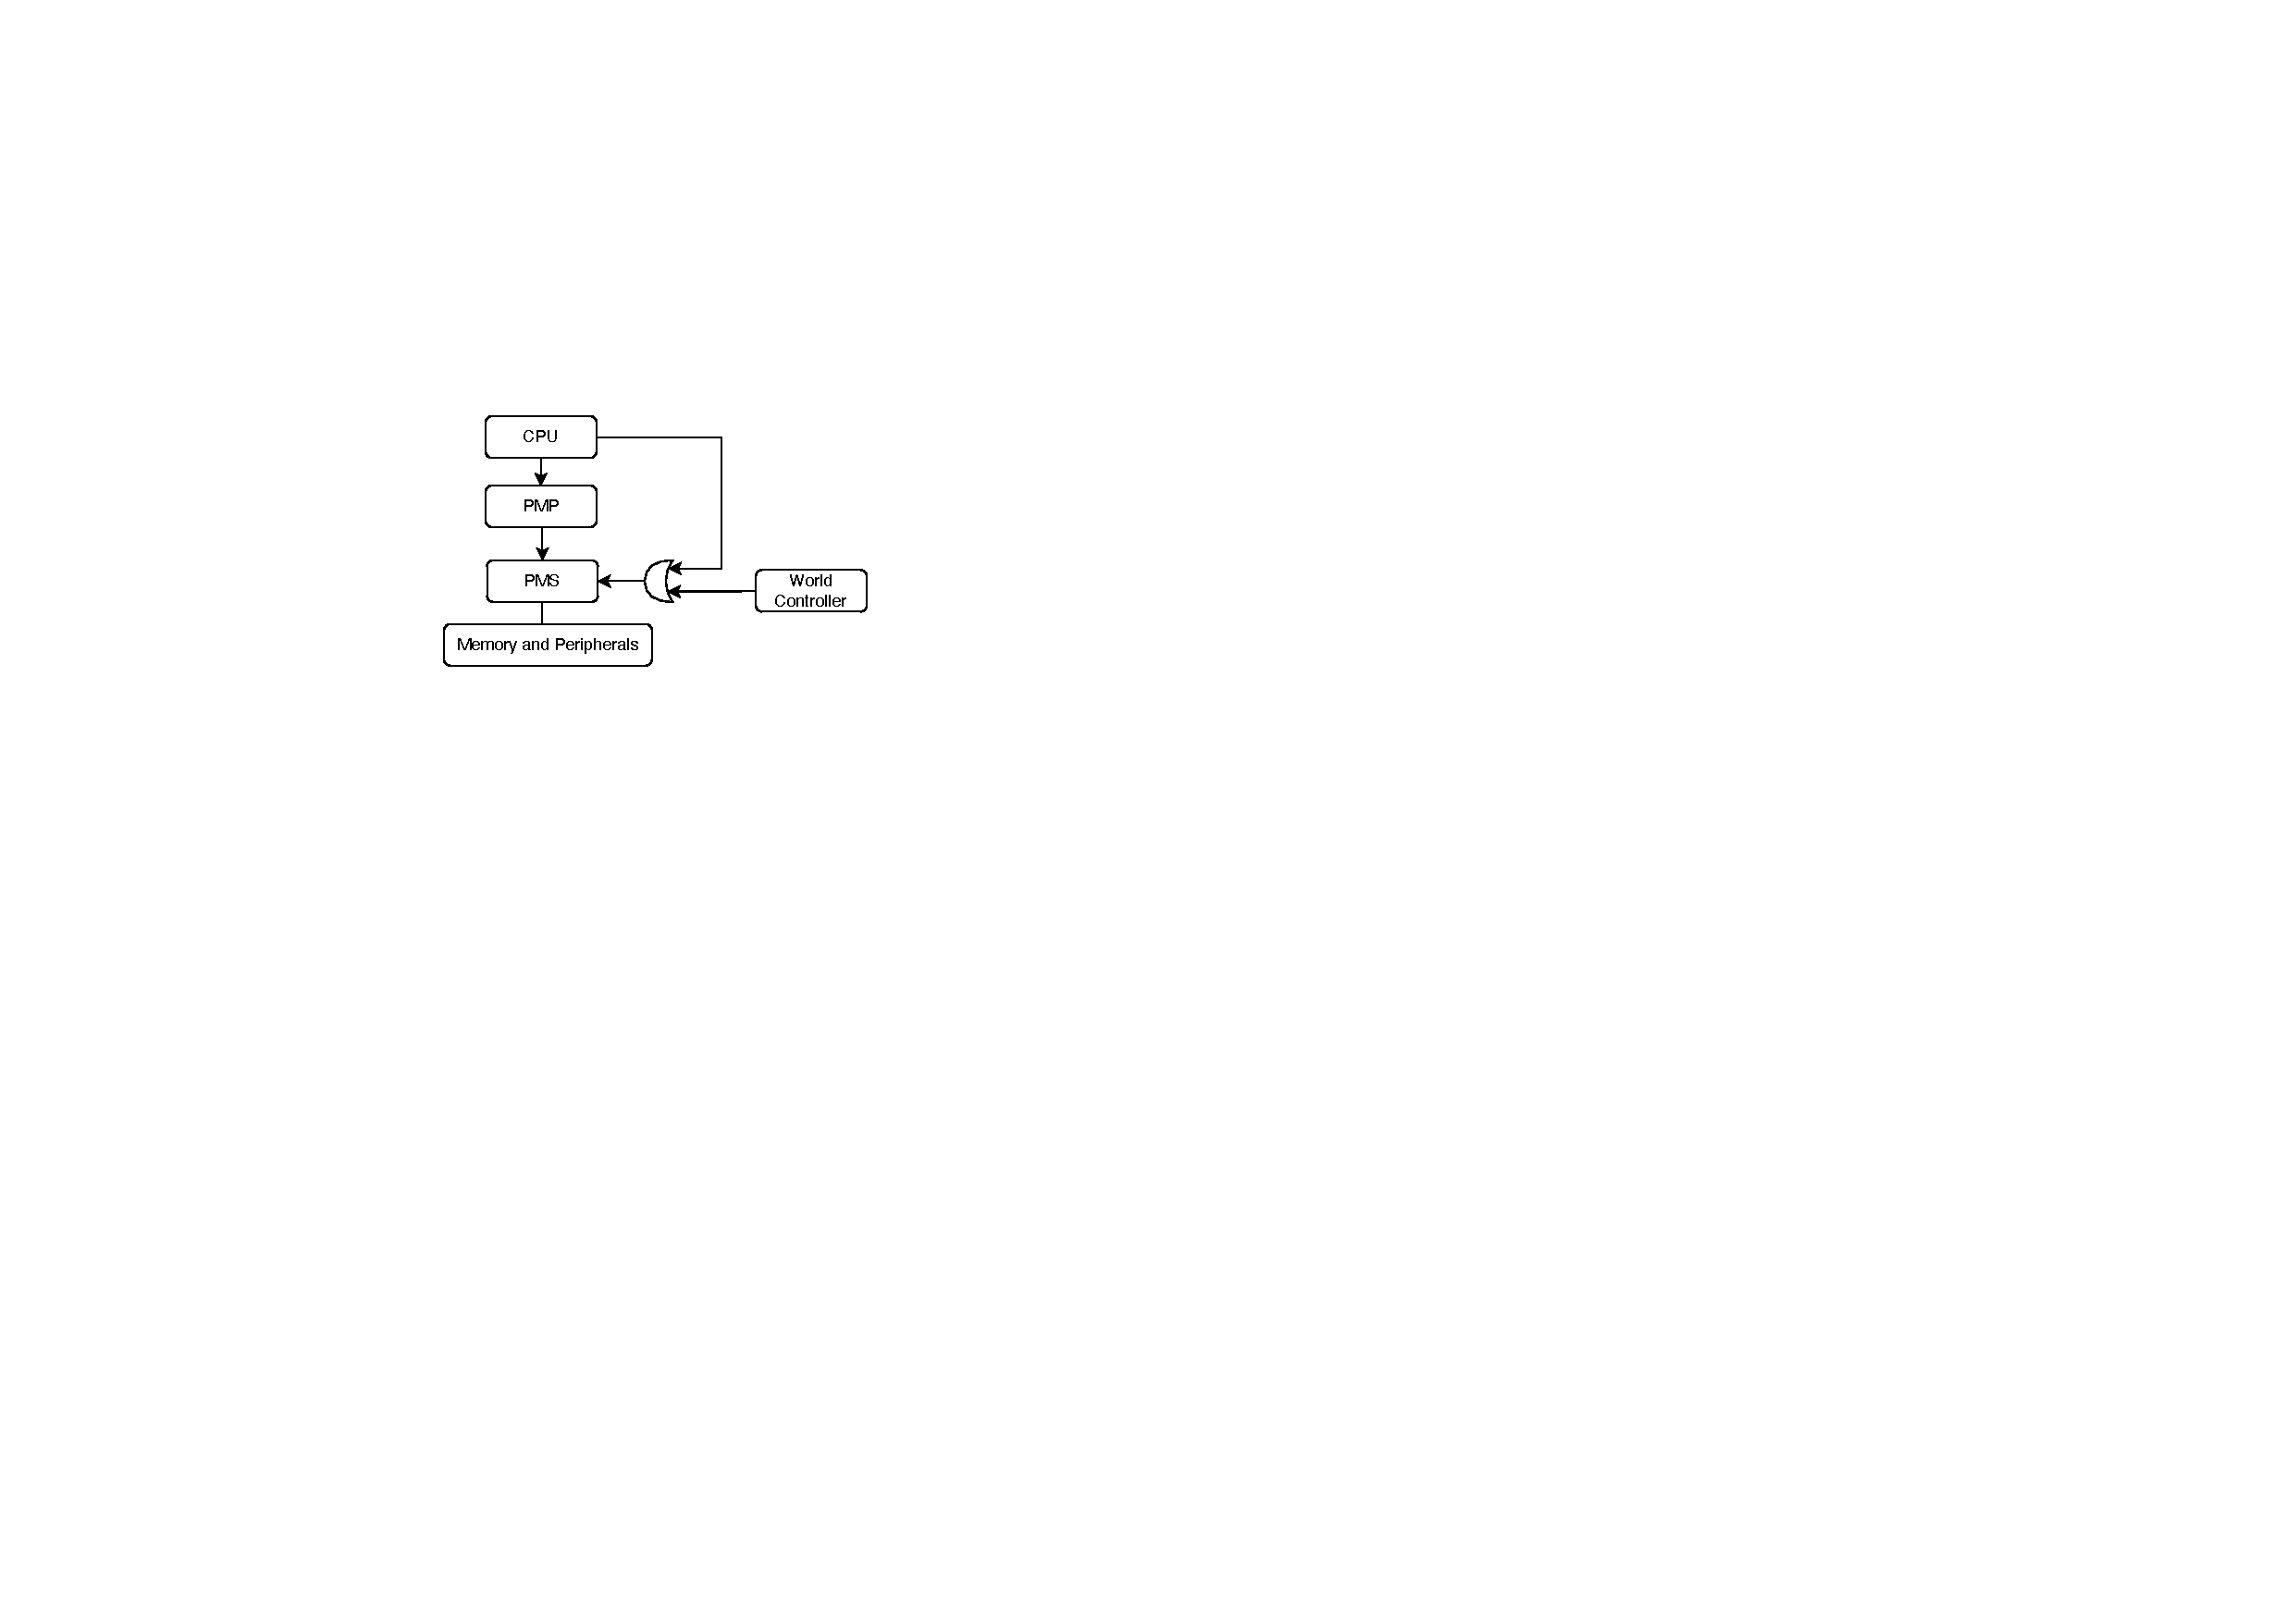
\includegraphics[width=0.6\textwidth]{./08-PERMCTRL/figures/c3_pms_pmp_new.pdf}
        \caption{Permission Control Overview}
        \label{fig:pms_overview}
    \end{figure}


For details about PMP, please refer to Section \ref{sec:riscvcpu-pmp-overview} in Chapter \ref{mod:riscvcpu} \textit{\nameref{mod:riscvcpu}}. For details about World Controller, please refer to Chapter \ref{mod:wctrl} \textit{\nameref{mod:wctrl}}. This chapter only describes \chipname{}'s PMS mechanism.

%%%%%%%%%%%%%%%%
%%% Features %%%
%%%%%%%%%%%%%%%%

\section{Features}

\chipname{}'s extended permission control mechanism supports:

\begin{itemize}
    \item Independent access management in a privileged environment and unprivileged environment
    \item Independent access management to internal memory, including
    \begin{itemize}
        \item CPU access to internal memory
        \item GDMA access to internal memory
    \end{itemize}
    \item Independent access management to external memory, including
    \begin{itemize}
        \item CPU to external memory via SPI1
        \item CPU to external memory via Cache
    \end{itemize}
    \item Independent access management to peripheral regions, including
    \begin{itemize}
        \item CPU access to peripheral regions
        \item Interrupt upon unsupported access alignment
    \end{itemize}
    \item Address splitting for more flexible access management
    \item Register locks to secure the integrity of access management related registers
    \item Interrupt upon unauthorized access
\end{itemize}


%%%%%%%%%%%%%%%%%%%%%%%%%%%%%%
%%% Functional Description %%%
%%%%%%%%%%%%%%%%%%%%%%%%%%%%%%


\section{Privileged Environment and Unprivileged Environment}

During PMS check, \chipname{} chip:
\begin{itemize}
    \item When in the privileged environment: check the permission configuration registers for the privileged environment
    \item When not in the unprivileged environment: check the permission configuration registers for the unprivileged environment
\end{itemize}

Users can choose either of these two ways below to enter the chip into privileged environment:
\begin{itemize}
    \item By configuring the world controller
    \begin{itemize}
        \item Switching to Secure world: entering the privileged environment
        \item Switching to Non-secure world: entering the unprivileged environment
    \end{itemize}
    \item By configuring the privileged level of the 32-bit RISC-V CPU:
    \begin{itemize}
        \item Switching to Machine mode: entering the privileged environment
        \item Switching to User mode: entering the unprivileged environment
    \end{itemize}
\end{itemize}


Users can configure \hyperref[fielddesc:PMSPRIVILEGEMODESEL]{PMS\_PRIVILEGE\_MODE\_SEL} to choose between the above-mentioned two ways to enter the chip into privileged environment:

\begin{itemize}
    \item 0 (Default): via configuring the world controller. See details in Chapter \ref{mod:wctrl} \textit{\nameref{mod:wctrl}}.
    \item 1: via configuring the CP's privileged level. See details in Chapter \ref{mod:riscvcpu} \textit{\nameref{mod:riscvcpu}}.
\end{itemize}

The following sections introduce how to configure the permission to different areas in the privileged environment and the unprivileged environment.

\section{Internal Memory}

\chipname{} has the following types of internal memory:
\begin{itemize}
    \item ROM: 384 KB in total, including 256 KB Internal ROM0 and 128 KB Internal ROM1
    \item SRAM: 400 KB in total, including 16 KB Internal SRAM0 and 384 KB Internal SRAM1
    \item RTC FAST Memory: 8 KB in total, which can be further split into two regions each with independent permission configuration
\end{itemize}

This section describes how to configure the permission to each type of \chipname{}'s internal memory.

\subsection{ROM}\label{sec:permctrl-PC-for-ROM}

\chipname{}'s ROM can be accessed by CPU's instruction bus (IBUS) and data bus (DBUS) when configured. The ROM ranges accessible for IBUS and DBUS respectively are listed in Table  \ref{tab:permctrl-ROM_block_address}.

\begin{table}[H]
    \centering
    \caption{ROM Address}
    \label{tab:permctrl-ROM_block_address}

    \begin{tabular}{|*{5}{c|} }
    \hline
        \rowcolor{lightgray}
         & \multicolumn{2}{c|}{\textbf{IBUS Address}} & \multicolumn{2}{c|}{\textbf{DBUS Address}} \\\cline{2-5}
        \rowcolor{lightgray}
        \multirow{-2}*{\textbf{ROM}} & \textbf{Starting Address} & \textbf{Ending Address} & \textbf{Starting Address} & \textbf{Ending Address} \\\hline

        % table contents
        Internal ROM0  & 0x4000\_0000 & 0x4003\_FFFF & - & - \\\hline
        Internal ROM1  & 0x4004\_0000 & 0x4005\_FFFF & 0x3FF0\_0000 & 0x3FF1\_FFFF \\\hline
        \end{tabular}
    \end{table}


\chipname{} uses the registers listed in Table  \ref{tab:permctrl-rom_permconfig} to configure the instruction execution (X), write (W) and read (R) accesses of CPU's IBUS and DBUS, in User mode and Machine mode. Note that access configuration to ROM0 and ROM1 cannot be configured separately:

\begin{table}[H]
    \centering
    \caption{Access Configuration to ROM (ROM0 and ROM1)}
    \label{tab:permctrl-rom_permconfig}
    \begin{threeparttable}
    \begin{tabular}{|l|l|l|l|}
        \hline
        \rowcolor{lightgray}
        \textbf{Bus} & \textbf{Environment} & \textbf{Configuration Registers\tnote{A}}                         & \textbf{Access} \\ \hline
                     & Privileged      & \hyperref[regdesc:PMSCOREXIRAM0PMSCONSTRAIN2REG]{PMS\_CORE\_X\_IRAM0\_PMS\_CONSTRAIN\_2\_REG   {[}20:18{]}}\tnote{B} & X/W/R           \\ \cline{2-4}
        \multirow{-2}{*}{IBUS} & Unprivileged & \hyperref[regdesc:PMSCOREXIRAM0PMSCONSTRAIN1REG]{PMS\_CORE\_X\_IRAM0\_PMS\_CONSTRAIN\_1\_REG {[}20:18{]}}\tnote{B}    & X/W/R \\ \hline
                     & Privileged      & \hyperref[regdesc:PMSCOREXDRAM0PMSCONSTRAIN1REG]{PMS\_CORE\_X\_DRAM0\_PMS\_CONSTRAIN\_1\_REG   {[}25:24{]}}\tnote{C} & W/R             \\ \cline{2-4}
        \multirow{-2}{*}{DBUS} & Unprivileged & \hyperref[regdesc:PMSCOREXDRAM0PMSCONSTRAIN1REG]{PMS\_CORE\_X\_DRAM0\_PMS\_CONSTRAIN\_1\_REG   {[}27:26{]}} & W/R   \\ \hline

        \end{tabular}
        \begin{tablenotes}
        \item[A] 1: with access; 0: without access
        \item[B] For example, configuring this field to 0b101 indicates CPU's IBUS is granted instruction execution and read accesses but not write access to ROM in the unprivileged environment.
        \item[C] For example, configuring this field to 0b01 indicates CPU's DBUS is granted read access but not write access to ROM in privileged environment.
        \end{tablenotes}
     \end{threeparttable}
    \end{table}

\subsection{SRAM}

\chipname{}'s SRAM can be accessed by CPU's instruction bus (IBUS) and data bus (DBUS) when configured. The SRAM address ranges accessible for IBUS and DBUS respectively are listed in Table  \ref{tab:permctrl-SRAM_block_address}.

\begin{table}[H]
    \centering
    \caption{SRAM Address}
    \label{tab:permctrl-SRAM_block_address}
    \begin{tabular}{ |*{6}{c|}}
    \hline
        \rowcolor{lightgray}
        & & \multicolumn{2}{c|}{\textbf{IBUS Address}} & \multicolumn{2}{c|}{\textbf{DBUS Address}} \\\cline{3-6}
        \rowcolor{lightgray}
        \multirow{-2}*{\textbf{SRAM}} & \multirow{-2}*{\textbf{Block}} & \textbf{Starting Address} & \textbf{Ending Address} & \textbf{Starting Address} & \textbf{Ending Address} \\\hline
        % table contents
        \multirow{1}*{Internal SRAM0}  & - & 0x4037\_C000 & 0x4037\_FFFF & - & - \\\hline
    \multirow{3}*{Internal SRAM1}
        & Block0 & 0x4038\_0000 & 0x4039\_FFFF & 0x3FC8\_0000 & 0x3FC9\_FFFF \\\cline{2-6}
        & Block1 & 0x403A\_0000 & 0x403B\_FFFF & 0x3FCA\_0000 & 0x3FCB\_FFFF \\\cline{2-6}
        & Block2 & 0x403C\_0000 & 0x403D\_FFFF & 0x3FCC\_0000 & 0x3FCD\_FFFF \\\hline
        \end{tabular}
    \end{table}

Here, we will first introduce how to configure the permission to Internal SRAM0 and then Internal SRAM1.

\subsubsection{Internal SRAM0 Access Configuration}\label{sec:permctrl_sram0}

\chipname{}'s Internal SRAM0 can be allocated to either CPU or ICACHE.

Users can configure \hyperref[fielddesc:PMSINTERNALSRAMUSAGECPUCACHE]{PMS\_INTERNAL\_SRAM\_USAGE\_CPU\_CACHE} to allocate \chipname{}'s Internal SRAM0 to either CPU or ICACHE:
\begin{itemize}
    \item 1: CPU
    \item 0: ICACHE
\end{itemize}

When the Internal SRAM0 is allocated to CPU, \chipname{} uses the registers listed in Table \ref{tab:permctrl-sram0_permconfig} to configure the instruction execution (X), write (W) and read (R) accesses of CPU's IBUS, in the privileged environment and the unprivileged environment:


\begin{table}[H]
    \centering
    \caption{Access Configuration to Internal SRAM0}
    \label{tab:permctrl-sram0_permconfig}
    \begin{threeparttable}
    \begin{tabular}{ |l|l|l|l|}
    \hline
        \rowcolor{lightgray}
        \textbf{Bus\tnote{A}} & \textbf{Environment} & \textbf{Configuration Registers\tnote{B}} & \textbf{Access} \\\hline
        \multirow{2}*{IBUS} & Privileged    &
        \scriptsize\hyperref[fielddesc:PMSCOREXIRAM0PMSCONSTRAINSRAMMMODECACHEDATAARRAYPMS0]{PMS\_CORE\_X\_IRAM0\_PMS\_CONSTRAIN\_SRAM\_M\_MODE\_CACHEDATAARRAY\_PMS\_0}\tnote{C} & X/W/R \\\cline{2-4}
                            & Unprivileged & \scriptsize\hyperref[fielddesc:PMSCOREXIRAM0PMSCONSTRAINSRAMUMODECACHEDATAARRAYPMS0]{PMS\_CORE\_X\_IRAM0\_PMS\_CONSTRAIN\_SRAM\_U\_MODE\_CACHEDATAARRAY\_PMS\_0 } & X/W/R \\\hline
        \end{tabular}
        \begin{tablenotes}
            \item[A] To access the Internal SRAM0, CPU must be configured with both the usage permission and respective access permission.
            \item[B] 1: with access; 0: without access
            \item[C] For example, configuring this field to 0b101 indicates CPU's IBUS is granted with instruction execution and read accesses but not write access to SRAM0 in the privileged environment.
        \end{tablenotes}
        \end{threeparttable}
    \end{table}

\subsubsection{Internal SRAM1 Access Configuration}\label{sec:permctrl_sram1}

\chipname{}'s Internal SRAM1 includes Block0 \verb+~+ Block2 (see details in Table \ref{tab:permctrl-SRAM_block_address}) and can be:
\begin{itemize}
    \item Accessed by CPU's DBUS, IBUS and GDMA at the same time
    \item Further split into up to 6 regions with independent access management for more flexible permission control.
\end{itemize}

\chipname{}'s Internal SRAM1 can be further split into up to 6 regions with 5 split lines. Users can configure different access to each region independently.

To be more specific, the Internal SRAM1 can be first split into Instruction Region and Data Region by IRam0\_DRam0\_split\_line:
\begin{itemize}
    \item Instruction Region:
    \begin{itemize}
    \item Then the Instruction Region should be only configured to be accessed by IBUS;
    \item And can be further split into three split regions by IRam0\_split\_line\_0 and IRam0\_split\_line\_1.
    \end{itemize}
    \item Data Region:
    \begin{itemize}
        \item The Data Region should be only configured to be accessed by DBUS;
        \item And can be further split into three split regions by DRam0\_split\_line\_0 and DRam0\_split\_line\_1.
    \end{itemize}
\end{itemize}

See illustration in Figure \ref{fig:permctrl_region_split} and Table \ref{tab:permctrl_region_split} below.

\begin{figure}[H]
        \centering
        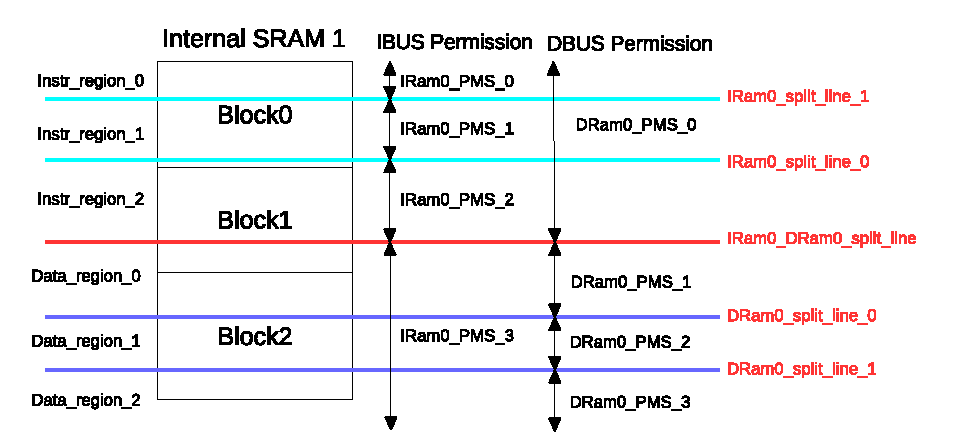
\includegraphics[width=0.7\textwidth]{./08-PERMCTRL/figures/split_line.eps}
        \caption{Split Lines for Internal SRAM1}
        \label{fig:permctrl_region_split}
    \end{figure}

\begin{table}[H]
\caption{Internal SRAM1 Split Regions}
\label{tab:permctrl_region_split}
\centering
\begin{threeparttable}
\begin{tabular}{|L{3cm}|L{6cm}|L{6cm}|}
\hline
\rowcolor{lightgray}
\textbf{Internal Memory \tnote{A}}                     & \textbf{Instruction / Data Regions}                                & \textbf{Split Regions\tnote{B}}             \\ \hline
\multirow{6}{*}{SRAM1} & \multirow{3}{*}{Instruction Region} & Instr\_Region\_0 \\ \cline{3-3}
                       &                                     & Instr\_Region\_1 \\ \cline{3-3}
                       &                                     & Instr\_Region\_2 \\ \cline{2-3}
                       & \multirow{3}{*}{Data   Region}      & Data\_Region\_0  \\ \cline{3-3}
                       &                                     & Data\_Region\_1  \\ \cline{3-3}
                       &                                     & Data\_Region\_2  \\ \hline
\end{tabular}
    \begin{tablenotes}
        \item[A] Access to each split region can be configured independently. See details in Table \ref{tab:permctrl_sram1_inst_permsplit} and \ref{tab:permctrl_sram1_data_permsplit}.
        \item[B] See the description below on how to configure the split lines.
    \end{tablenotes}
\end{threeparttable}
\end{table}

\subparagraph{Internal SRAM1 Split Regions}\label{sec:permctrl-split-line}

\chipname{} allows users to configure the split lines to their needs with registers below:
\begin{itemize}
    \item Split line to split the Instruction and Data regions (IRam0\_DRam0\_split\_line):
    \begin{itemize}
        \item \hyperref[regdesc:PMSCOREXIRAM0DRAM0DMASPLITLINECONSTRAIN1REG]{PMS\_CORE\_X\_IRAM0\_DRAM0\_DMA\_SPLIT\_LINE\_CONSTRAIN\_1\_REG}
    \end{itemize}
    \item The first split line to further split the Instruction Region (IRam0\_split\_line\_0):
    \begin{itemize}
        \item \hyperref[regdesc:PMSCOREXIRAM0DRAM0DMASPLITLINECONSTRAIN2REG]{PMS\_CORE\_X\_IRAM0\_DRAM0\_DMA\_SPLIT\_LINE\_CONSTRAIN\_2\_REG}
    \end{itemize}
    \item The second split line to further split the Instruction Region (IRam0\_split\_line\_1):
    \begin{itemize}
        \item \hyperref[regdesc:PMSCOREXIRAM0DRAM0DMASPLITLINECONSTRAIN3REG]{PMS\_CORE\_X\_IRAM0\_DRAM0\_DMA\_SPLIT\_LINE\_CONSTRAIN\_3\_REG}
    \end{itemize}
    \item The first split line to further split the data Region (DRam0\_split\_line\_0):
    \begin{itemize}
        \item \hyperref[regdesc:PMSCOREXIRAM0DRAM0DMASPLITLINECONSTRAIN4REG]{PMS\_CORE\_X\_IRAM0\_DRAM0\_DMA\_SPLIT\_LINE\_CONSTRAIN\_4\_REG}
    \end{itemize}
    \item The second split line to further split the data Region (DRam0\_split\_line\_1):
    \begin{itemize}
        \item \hyperref[regdesc:PMSCOREXIRAM0DRAM0DMASPLITLINECONSTRAIN5REG]{PMS\_CORE\_X\_IRAM0\_DRAM0\_DMA\_SPLIT\_LINE\_CONSTRAIN\_5\_REG}
    \end{itemize}
\end{itemize}

When configuring the split lines,
\begin{enumerate}
    \item First configure the block in which the split line is by:
    \begin{itemize}
        \item Configuring the Category\_\regindex{x} field for the block in which the split line is to 0x1 or 0x2 (no difference)
        \item Configuring the Category\_0 \verb+~+ Category\_\regindex{x-1} fields for all the preceding blocks to 0x0
        \item Configuring the Category\_\regindex{x+1} \verb+~+ Category\_2 fields for all blocks afterwards to 0x3
    \end{itemize}
        For example, assuming you want to configure the split line in Block1, then first configure the Category\_1 field for Block1 to 0x1 or 0x2; configure the Category\_0 for Block0 to 0x0; and configure the Category\_2 for Block2 to 0x3 (see illustration in Figure \ref{fig:PERMCTRL_category_config}). On the other hand, when reading 0x1 or 0x2 from Category\_1, then you know the split line is in Block1.
    \item Configure the position of the split line inside the configured block by:
    \begin{itemize}
        \item Writing the [16:9] bits of the actual address at which you want to split the memory to the \hyperref[fielddesc:PMSCOREXIRAM0SRAMLINE0SPLITADDR]{SPLITADDR} field for the block in which the split line is.
        \item Note that the split address must be aligned to 512 bytes, meaning you can only write the integral multiples of 0x200 to the \hyperref[fielddesc:PMSCOREXIRAM0SRAMLINE0SPLITADDR]{SPLITADDR} field.
    \end{itemize}
        For example, if you want to split the instruction region at 0x3fc88000, then write the [16:9] bits of this address, which is 0b01000000, to \hyperref[fielddesc:PMSCOREXIRAM0SRAMLINE0SPLITADDR]{SPLITADDR}.
    \item The split address applies to both IBUS and DBUS address. For example, DBUS address 0x3fc88000 and IBUS address 0x40388000 indicate the same location in SRAM1. The split address for both buses is [16:9].
\end{enumerate}

\begin{figure}[H]
        \centering
        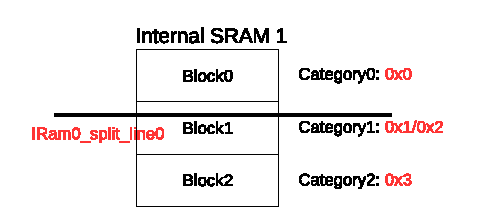
\includegraphics[width=0.5\textwidth]{./08-PERMCTRL/figures/split_line_category.eps}
        \caption{An illustration of Configuring the Category fields}
        \label{fig:PERMCTRL_category_config}
\end{figure}

Note the following points when configuring the split lines:

 \begin{itemize}
     \item Position:
     \begin{itemize}
         \item The split line that splitting the Instruction Region and Data Region can be configured anywhere inside Internal SRAM1.
         \item The two split lines further splitting the Instruction Region into 3 split regions must stay inside the Instruction Region.
         \item The two split lines further splitting the Data Region into 3 split regions must stay inside the Data Region.
     \end{itemize}
     \item Spilt lines can overlap with each other. For example,
     \begin{itemize}
         \item When the two split lines inside the Data Region are not overlapping with each other, then the Data Region is split into 3 split regions
         \item When the two split lines inside the Data Region are overlapping with each other, then the Data Region is only split into 2 split regions
         \item When the two split lines inside the Data Region are not only overlapping with each other but also with the split line that splits the Data Region and the Instruction Region, then the Data Region is not split at all and only has one region.
     \end{itemize}
     \end{itemize}

\subparagraph{Access Configuration}

After configuring the split lines, users can then use the registers described in the Table \ref{tab:permctrl_sram1_inst_permsplit} and Table \ref{tab:permctrl_sram1_data_permsplit} below to configure the access of CPU's IBUS, DBUS and GDMA peripherals, in the privileged environment and the unprivileged environment, to these split regions independently.

\begin{table}[H]
    \centering
    \caption{Access Configuration to the Instruction Region of Internal SRAM1}
    \label{tab:permctrl_sram1_inst_permsplit}

    \begin{threeparttable}
    \begin{tabular}{ |l|L{3CM}|l|c|c|c|l| }
    \hline
    \rowcolor{lightgray}
        & & & \multicolumn{3}{c|}{\textbf{Instruction Region}} &  \\\cline{4-6}
    \rowcolor{lightgray}
    \multirow{-2}*{\textbf{Buses}}   & \multirow{-2}*{\textbf{Environment}} & \multirow{-2}*{\textbf{Configuration Registers}} & \scriptsize{\textbf{instr\_region\_0}} & \scriptsize{\textbf{instr\_region\_1}} & \scriptsize{\textbf{instr\_region\_2}} & \multirow{-2}*{\textbf{Access}}   \\\hline
    \multirow{2}*{IBUS}             & Privileged         & \scriptsize{\hyperref[regdesc:PMSCOREXIRAM0PMSCONSTRAIN2REG]{PMS\_CORE\_X\_IRAM0\_PMS\_CONSTRAIN\_2\_REG}} & [2:0] & [5:3] & [8:6] & X/W/R \\\cline{2-7}
                                    &  Unprivileged      & \scriptsize{\hyperref[regdesc:PMSCOREXIRAM0PMSCONSTRAIN1REG]{PMS\_CORE\_X\_IRAM0\_PMS\_CONSTRAIN\_1\_REG}} & [2:0] & [5:3] & [8:6] & X/W/R \\\hline

     \multirow{2}*{DBUS}            & Privileged        &                                                                             & \multicolumn{3}{c|}{[13:12]\tnote{A}} & W/R \\ \cline{2-2} \cline{4-7}
                                    &  Unprivileged      & \multirow{-2}*{\scriptsize{\hyperref[regdesc:PMSCOREXDRAM0PMSCONSTRAIN1REG]{PMS\_Core\_X\_DRAM0\_PMS\_CONSTRAIN\_1\_REG}}}      & \multicolumn{3}{c|}{[1:0]\tnote{A}}  & W/R \\\hline
    GDMA  \tnote{C}                      & \regindex{XX} Peripherals    \tnote{D}           & \scriptsize{\hyperref[regdesc:PMSDMAAPBPERISPI2PMSCONSTRAIN1REG]{PMS\_DMA\_APBPERI\_\regindex{XX}\_PMS\_CONSTRAIN\_1\_REG}}  &   \multicolumn{3}{c|}{[1:0]\tnote{B}}   & W/R \\\hline

    \end{tabular}
        \begin{tablenotes}
            \item [A] Configure DBUS' access to the Instruction Region. However, it's recommended to configure these bits to 0.
            \item [B] Configure GDMA's access to the Instruction Region. However, it's recommended to configure these bits to 0.
            \item [C] GMDA doesn't support the privileged environment and unprivileged environment.
            \item [D] \chipname{} has 6 peripherals, including SPI2, UCHI0, I2S, AES, SHA, ADC, which can access Internal SRAM1 via GDMA. Each peripherals can be configured with different access to the Internal SRAM1 independently.

        \end{tablenotes}
     \end{threeparttable}
    \end{table}

\begin{table}[H]
    \centering
    \caption{Access Configuration to the Data Region of Internal SRAM1}
    \label{tab:permctrl_sram1_data_permsplit}

    \begin{threeparttable}
    \begin{tabular}{ |l|L{3CM}|l|c|c|c|l| }
    \hline
    \rowcolor{lightgray}
        & & & \multicolumn{3}{c|}{\textbf{Data Region}} &  \\\cline{4-6}
    \rowcolor{lightgray}
    \multirow{-2}*{\textbf{Buses}}   & \multirow{-2}*{\textbf{Environment}} & \multirow{-2}*{\textbf{Configuration Registers}} & \scriptsize{\textbf{data\_region\_0}} & \scriptsize{\textbf{data\_region\_1}} & \scriptsize{\textbf{data\_region\_2}} & \multirow{-2}*{\textbf{Access}}   \\\hline
         \multirow{2}*{IBUS}            & Privileged        &  \scriptsize{\hyperref[regdesc:PMSCOREXIRAM0PMSCONSTRAIN2REG]{PMS\_CORE\_X\_IRAM0\_PMS\_CONSTRAIN\_2\_REG}}                                                                                        & \multicolumn{3}{c|}{[11:9]\tnote{A}}  & X/W/R \\ \cline{2-7}
                                    & Unprivileged      & \scriptsize{\hyperref[regdesc:PMSCOREXIRAM0PMSCONSTRAIN1REG]{PMS\_CORE\_X\_IRAM0\_PMS\_CONSTRAIN\_1\_REG}}      & \multicolumn{3}{c|}{[11:9]\tnote{A}}  & X/W/R \\\hline
    \multirow{2}*{DBUS}             & Privileged        &                                                                                    & [3:2] & [5:4] & [7:6] & W/R \\\cline{2-2} \cline{4-7}
                                    & Unprivileged      & \multirow{-2}*{\scriptsize{\hyperref[regdesc:PMSCOREXDRAM0PMSCONSTRAIN1REG]{PMS\_Core\_X\_DRAM0\_PMS\_CONSTRAIN\_1\_REG}}} & [15:14] & [17:16] & [19:18] & W/R \\\hline
    GDMA \tnote{B}                   & \regindex{XX} Peripherals\tnote{C}              & \scriptsize{\hyperref[regdesc:PMSDMAAPBPERISPI2PMSCONSTRAIN1REG]{PMS\_DMA\_APBPERI\_\regindex{XX}\_PMS\_CONSTRAIN\_1\_REG}}  &  [3:2] & [5:4] & [7:6]    & W/R \\\hline

    \end{tabular}
        \begin{tablenotes}
            \item [A] Configure IBUS' access to the Data Region. However, it's recommended to configure these bits to 0.
            \item [B] GMDA doesn't support the privileged environment and the unprivileged environment.
            \item [C] \chipname{} has six peripherals, including SPI2, UCHI0, I2S, AES, SHA, ADC, which can access Internal SRAM1 via GDMA. Each peripheral can be configured with different access to the Internal SRAM1 independently.
            \end{tablenotes}
     \end{threeparttable}
\end{table}

For details on how to configure the split lines, see Section \ref{sec:permctrl-split-line}.

\begin{tiplisting}
If enabled, the permission control module watches all the memory access and fires the panic handler if a permission violation is detected. This feature automatically splits the SRAM memory into data and instruction segments and sets Read/Execute permissions for the instruction part (below given splitting address) and Read/Write permissions for the data part (above the splitting address). The memory protection is effective on all access through the IRAM0 and DRAM0 buses.
See details, see  {\it{\href{https://docs.espressif.com/projects/esp-idf/zh_CN/v4.3-beta1/esp32c3/api-reference/kconfig.html#memory-protection}{ESP-IDF api-reference Memory protection}}}.
\end{tiplisting}


\subsection{RTC FAST Memory}

\chipname{}'s RTC FAST Memory is 8 KB. See the address of RTC FAST Memory below:

\begin{longtable}[c]{ |l|l|l| }
\caption{RTC FAST Memory Address}
\label{tab:fast-memory-address}
\\\hline
\rowcolor{lightgray}
    \textbf{Memory} &  \textbf{Starting Address}  &  \textbf{Ending Address}\\
    \hline
    RTC FAST Memory          & 0x5000\_0000 &  0x5000\_1FFF   \\
    \hline
\end{longtable}


\chipname{}'s RTC FAST Memory can be further split into 2 regions. Each split region can be configured independently with different access.

The Register for configuring the split line is described below:

\begin{table}[H]
    \centering
    \caption{Split RTC FAST Memory into the Higher Region and the Lower Region}
    \label{tab:rtc_fast_mem_split}
    \begin{threeparttable}
    \begin{tabular}{|l|l|l|} \hline
    \rowcolor{lightgray}
     & \textbf{Privileged Environment} & \textbf{Unprivileged Environment} \\\hline
    \textbf{Split Lines Configuration Register}\tnote{1} & \hyperref[regdesc:PMSCORE0PIFPMSCONSTRAIN9REG]{PIF\_PMS\_CONSTRAN\_9\_REG} [10:0]  & \hyperref[regdesc:PMSCORE0PIFPMSCONSTRAIN9REG]{PIF\_PMS\_CONSTRAN\_9\_REG} [21:11] \\\hline
    \end{tabular}
        \begin{tablenotes}
        \item[1] The word offset from the RTC FAST Memory base address should be used when configuring the split address. For example, if you want to split the RTC FAST Memory at 0x5000\_1000, then write 0x400 (0x1000$>>$2) to this register.
        \end{tablenotes}
    \end{threeparttable}
\end{table}

Access configuration for the higher and lower regions of the RTC FAST Memory is described below:
\begin{table}[H]
    \centering
    \caption{Access Configuration to the RTC FAST Memory}
    \label{tab:rtc_fast_mem_split_access}
    \begin{threeparttable}
    \begin{tabular}{|l|c|l|l|l|} \hline
    \rowcolor{lightgray}
     &\textbf{RTC}  & \multicolumn{2}{c|}{\textbf{Configuration Registers}}& \\\cline{3-4}
    \rowcolor{lightgray}
    \multirow{-2}*{\textbf{Bus}}   & \textbf{FAST Memory} & \textbf{Privileged Environment} & \textbf{Unprivileged Environment} & \multirow{-2}*{\textbf{Access}\tnote{A}} \\\hline
     Peri Bus    & Higher Region                       &   \hyperref[regdesc:PMSCORE0PIFPMSCONSTRAIN10REG]{PIF\_PMS\_CONSTRAN\_10\_REG} [5:3] \tnote{B}               &    \hyperref[regdesc:PMSCORE0PIFPMSCONSTRAIN10REG]{PIF\_PMS\_CONSTRAN\_10\_REG} [11:9]  & \\\cline{2-4}
      (PIF) & Lower Region & \hyperref[regdesc:PMSCORE0PIFPMSCONSTRAIN10REG]{PIF\_PMS\_CONSTRAN\_10\_REG} [2:0] & \hyperref[regdesc:PMSCORE0PIFPMSCONSTRAIN10REG]{PIF\_PMS\_CONSTRAN\_10\_REG} [8:6]  & \multirow{-2}*{X/R/W}  \\\hline
    \end{tabular}
        \begin{tablenotes}
        \item[A] 1: with access; 0: without access
        \item[B] For example, configuring this field to 0b101 indicates CPU's peripheral (PIF) bus is granted with the instruction execution and read accesses but not the read access in the privileged environment to the higher region of RTC FAST Memory.
        \end{tablenotes}
    \end{threeparttable}
\end{table}

\section{Peripherals}
\subsection{Access Configuration}\label{sec:permctrl-peri-address}

\chipname{}'s CPU can be configured with different read (R) and write (W) accesses to most of its modules and peripherals independently, in the privileged environment and in the unprivileged environment, by configuring respective registers \newline (\hyperref[regdesc:PMSCORE0PIFPMSCONSTRAIN1REG]{PMS\_CORE\_0\_PIF\_PMS\_CONSTRAN\_\regindex{n}\_REG}).

Notes on \hyperref[regdesc:PMSCORE0PIFPMSCONSTRAIN1REG]{PMS\_CORE\_0\_PIF\_PMS\_CONSTRAN\_\regindex{n}\_REG}:
\begin{itemize}
    \item \regindex{n} can be 1 \verb+~+ 8, in which 1 \verb+~+ 4 are for the privileged environment and 5 \verb+~+ 8 are for the unprivileged environment.
\end{itemize}

For example, users can configure  \hyperref[regdesc:PMSCORE0PIFPMSCONSTRAIN1REG]{PMS\_CORE\_0\_PIF\_PMS\_CONSTRAIN\_1\_REG [1:0]} to 0x2, meaning CPU is granted with read access but not write access in the privileged environment to UART0. In this case, CPU won't be able to modify the UART0's internal registers when in the privileged environment.
\begin{ThreePartTable}

\begin{TableNotes}
\item[1]: This is shared by more than one peripherals.
\item[2]: Accelerators: AES, SHA, RSA, Digital Signatures, HMAC
\item[3]: Access: R/W
\item[4]: ** in the table replaces PMS\_CORE\_0\_PIF.
\end{TableNotes}

\begin{longtable}[c]{ |l|l|l|l| }
    \caption{Access Configuration of the Peripherals}
    \label{tab:sysreg-peripheral-controlling-bit1}
    \\\hline\rowcolor{lightgray}
    \textbf{Peripherals}    & \textbf{Privileged Environment} & \textbf{Unprivileged Environment} & \textbf{Bit}\tnote{3}\\\hline
    \endfirsthead
    \multicolumn{3}{c}{\bfseries \tablename\ \thetable{} -- cont'd from previous page}\\\hline
    \rowcolor{lightgray}
    \textbf{Peripherals}    & \textbf{Privileged Environment} & \textbf{Unprivileged Environment} & \textbf{Bit}\tnote{3}\\\hline
    \endhead
    \multicolumn{3}{r}{\textbf{Cont'd on next page}} \\
    \endfoot
    \insertTableNotes
    \endlastfoot
    GDMA  & **\_PMS\_CONSTRAN\_4\_REG & **\_PMS\_CONSTRAN\_8\_REG & [7:6] \\\hline
    eFuse Controller \& PMU\tnote{1} & **\_PMS\_CONSTRAN\_1\_REG & **\_PMS\_CONSTRAN\_5\_REG & [15:14] \\\hline
    IO\_MUX & **\_PMS\_CONSTRAN\_1\_REG & **\_PMS\_CONSTRAN\_5\_REG & [17:16] \\\hline
    GPIO & **\_PMS\_CONSTRAN\_1\_REG & **\_PMS\_CONSTRAN\_5\_REG & [7:6] \\\hline
    Interrupt Matrix & **\_PMS\_CONSTRAN\_4\_REG & **\_PMS\_CONSTRAN\_8\_REG & [21:20] \\\hline
    System Timer & **\_PMS\_CONSTRAN\_2\_REG & **\_PMS\_CONSTRAN\_6\_REG & [31:30] \\\hline
    Timer Group 0 & **\_PMS\_CONSTRAN\_2\_REG & **\_PMS\_CONSTRAN\_6\_REG & [27:26] \\\hline
    Timer Group 1 & **\_PMS\_CONSTRAN\_2\_REG & **\_PMS\_CONSTRAN\_6\_REG & [29:28] \\\hline
    System Registers & **\_PMS\_CONSTRAN\_4\_REG & **\_PMS\_CONSTRAN\_8\_REG & [17:16] \\\hline
    PMS Registers & **\_PMS\_CONSTRAN\_4\_REG & **\_PMS\_CONSTRAN\_8\_REG & [19:18] \\\hline
    Debug Assist & **\_PMS\_CONSTRAN\_4\_REG & **\_PMS\_CONSTRAN\_8\_REG & [27:26] \\\hline
    Accelerators\tnote{2} & **\_PMS\_CONSTRAN\_4\_REG & **\_PMS\_CONSTRAN\_8\_REG & [5:4] \\\hline
    Cache \& XTS\_AES\tnote{1} & **\_PMS\_CONSTRAN\_4\_REG & **\_PMS\_CONSTRAN\_8\_REG & [25:25] \\\hline
    UART 0 & **\_PMS\_CONSTRAN\_1\_REG & **\_PMS\_CONSTRAN\_5\_REG & [1:0] \\\hline
    UART 1 & **\_PMS\_CONSTRAN\_1\_REG & **\_PMS\_CONSTRAN\_5\_REG & [31:30] \\\hline
    SPI 0 & **\_PMS\_CONSTRAN\_1\_REG & **\_PMS\_CONSTRAN\_5\_REG & [5:4] \\\hline
    SPI 1 & **\_PMS\_CONSTRAN\_1\_REG & **\_PMS\_CONSTRAN\_5\_REG & [3:2] \\\hline
    SPI 2 & **\_PMS\_CONSTRAN\_3\_REG & **\_PMS\_CONSTRAN\_7\_REG & [1:0] \\\hline
    I2C 0 & **\_PMS\_CONSTRAN\_2\_REG & **\_PMS\_CONSTRAN\_6\_REG & [5:4] \\\hline
    I2S & **\_PMS\_CONSTRAN\_3\_REG & **\_PMS\_CONSTRAN\_7\_REG & [15:14] \\\hline
    USB OTG Core & **\_PMS\_CONSTRAN\_4\_REG & **\_PMS\_CONSTRAN\_8\_REG & [15:14] \\\hline
    Two-wire Automotive Interface & **\_PMS\_CONSTRAN\_3\_REG & **\_PMS\_CONSTRAN\_7\_REG & [11:10] \\\hline
    UHCI 0  & **\_PMS\_CONSTRAN\_2\_REG & **\_PMS\_CONSTRAN\_6\_REG & [7:6] \\\hline
    LED PWM Controller  & **\_PMS\_CONSTRAN\_2\_REG & **\_PMS\_CONSTRAN\_6\_REG & [17:16] \\\hline
    Remote Control Peripheral  & **\_PMS\_CONSTRAN\_2\_REG & **\_PMS\_CONSTRAN\_6\_REG & [11:10] \\\hline
    APB Controller & **\_PMS\_CONSTRAN\_3\_REG & **\_PMS\_CONSTRAN\_7\_REG & [5:4] \\\hline
    ADC Controller & **\_PMS\_CONSTRAN\_4\_REG & **\_PMS\_CONSTRAN\_8\_REG & [9:8] \\\hline
\end{longtable}
\end{ThreePartTable}

\subsection{Split Peripheral Regions into Split Regions}

On top of what described in the previous section, user can select one of \chipname{}'s peripheral region to split them into 7 regions (from Peri Region0 \verb+~+ Peri Region7) for more flexible permission control.

For example, the registers for \chipname{}'s GDMA controller are allocated as:
\begin{itemize}
    \item 3 sets of registers for each of 3 RX channel
    \item 3 sets of registers for each of 3 TX channel
    \item 1 set of registers for configuration
\end{itemize}

As seen above, GDMA's peripheral region is divided into 7 split regions (implemented in hardware), which can be configured with different permission independently, thus achieving independent permission control for each GDMA channel.

Users can configure CPU's read (R) and write (W) accesses to a specific split region (Peri Region\regindex{n}) in the privileged environment and in the unprivileged environment by configuring \hyperref[regdesc:PMSREGIONPMSCONSTRAIN1REG]{PMS\_REGION\_PMS\_CONSTRAN\_\regindex{n}\_REG}.

Notes on \hyperref[regdesc:PMSREGIONPMSCONSTRAIN1REG]{PMS\_REGION\_PMS\_CONSTRAN\_\regindex{n}\_REG}:
\begin{itemize}
    \item \regindex{n} can be 1\verb+~+10, in which    \begin{itemize}
        \item \hyperref[regdesc:PMSREGIONPMSCONSTRAIN1REG]{PMS\_REGION\_PMS\_CONSTRAN\_1\_REG} is for configuring CPU's permission in the privileged environment.
        \item \hyperref[regdesc:PMSREGIONPMSCONSTRAIN2REG]{PMS\_REGION\_PMS\_CONSTRAN\_2\_REG} is for configuring CPU's permission in the unprivileged environment.
        \item \hyperref[regdesc:PMSREGIONPMSCONSTRAIN3REG]{PMS\_REGION\_PMS\_CONSTRAN\_\regindex{n}\_REG} (\regindex{n} = 3\verb+~+10) are used to configuring the starting addresses for each Peri Regions. Note the starting address of each Peri Region is also the ending address of the previous Peri Region.
    \end{itemize}
\end{itemize}


\begin{table}[H]
    \centering
    \caption{Access Configuration of Peri Regions}
    \label{tab:perpheral_region_config}
    \begin{threeparttable}
    \begin{tabular}{ | l | l | l | l |}
    \hline
        \rowcolor{lightgray}
         & \textbf{Starting Address} & \multicolumn{2}{c|}{\textbf{Access Configuration}} \\\cline{3-4}
        \rowcolor{lightgray}
        \multirow{-2}*{\textbf{Peri Regions}} & \textbf{Configuration} & \textbf{Privileged Environment} & \textbf{Unprivileged Environment} \\\hline
        Peri Region0 & \scriptsize{\hyperref[regdesc:PMSREGIONPMSCONSTRAIN3REG]{PMS\_REGION\_PMS\_CONSTRAN\_3\_REG}} & \scriptsize{\hyperref[regdesc:PMSREGIONPMSCONSTRAIN1REG]{\hyperref[regdesc:PMSREGIONPMSCONSTRAIN1REG]{PMS\_REGION\_PMS\_CONSTRAN\_1\_REG}} [1:0]} & \scriptsize{\hyperref[regdesc:PMSREGIONPMSCONSTRAIN1REG]{PMS\_REGION\_PMS\_CONSTRAN\_2\_REG} [1:0]}\\\hline
        Peri Region1 & \scriptsize{\hyperref[regdesc:PMSREGIONPMSCONSTRAIN3REG]{PMS\_REGION\_PMS\_CONSTRAN\_4\_REG}} & \scriptsize{\hyperref[regdesc:PMSREGIONPMSCONSTRAIN1REG]{PMS\_REGION\_PMS\_CONSTRAN\_1\_REG} [3:2]} & \scriptsize{\hyperref[regdesc:PMSREGIONPMSCONSTRAIN1REG]{PMS\_REGION\_PMS\_CONSTRAN\_2\_REG} [3:2]}\\\hline
        Peri Region2 & \scriptsize{\hyperref[regdesc:PMSREGIONPMSCONSTRAIN3REG]{PMS\_REGION\_PMS\_CONSTRAN\_5\_REG}} & \scriptsize{\hyperref[regdesc:PMSREGIONPMSCONSTRAIN1REG]{PMS\_REGION\_PMS\_CONSTRAN\_1\_REG} [5:4]} & \scriptsize{\hyperref[regdesc:PMSREGIONPMSCONSTRAIN1REG]{PMS\_REGION\_PMS\_CONSTRAN\_2\_REG} [5:4]}\\\hline
        Peri Region3 & \scriptsize{\hyperref[regdesc:PMSREGIONPMSCONSTRAIN3REG]{PMS\_REGION\_PMS\_CONSTRAN\_6\_REG}} & \scriptsize{\hyperref[regdesc:PMSREGIONPMSCONSTRAIN1REG]{PMS\_REGION\_PMS\_CONSTRAN\_1\_REG} [7:6]} & \scriptsize{\hyperref[regdesc:PMSREGIONPMSCONSTRAIN1REG]{PMS\_REGION\_PMS\_CONSTRAN\_2\_REG} [7:6]}\\\hline
        Peri Region4 & \scriptsize{\hyperref[regdesc:PMSREGIONPMSCONSTRAIN3REG]{PMS\_REGION\_PMS\_CONSTRAN\_7\_REG}} & \scriptsize{\hyperref[regdesc:PMSREGIONPMSCONSTRAIN1REG]{PMS\_REGION\_PMS\_CONSTRAN\_1\_REG} [9:8]} & \scriptsize{\hyperref[regdesc:PMSREGIONPMSCONSTRAIN1REG]{PMS\_REGION\_PMS\_CONSTRAN\_2\_REG} [9:8]}\\\hline
        Peri Region5 & \scriptsize{\hyperref[regdesc:PMSREGIONPMSCONSTRAIN3REG]{PMS\_REGION\_PMS\_CONSTRAN\_8\_REG}} & \scriptsize{\hyperref[regdesc:PMSREGIONPMSCONSTRAIN1REG]{PMS\_REGION\_PMS\_CONSTRAN\_1\_REG} [11:10]} & \scriptsize{\hyperref[regdesc:PMSREGIONPMSCONSTRAIN1REG]{PMS\_REGION\_PMS\_CONSTRAN\_2\_REG} [11:10]}\\\hline
        Peri Region6\tnote{*} & \scriptsize{\hyperref[regdesc:PMSREGIONPMSCONSTRAIN3REG]{PMS\_REGION\_PMS\_CONSTRAN\_9\_REG}} & \scriptsize{\hyperref[regdesc:PMSREGIONPMSCONSTRAIN1REG]{PMS\_REGION\_PMS\_CONSTRAN\_1\_REG} [13:12]} & \scriptsize{\hyperref[regdesc:PMSREGIONPMSCONSTRAIN1REG]{PMS\_REGION\_PMS\_CONSTRAN\_2\_REG} [13:12]}\\\hline
    \end{tabular}
    \begin{tablenotes}
        \item[*] The ending address of Peri Region6 is configured by \hyperref[regdesc:PMSREGIONPMSCONSTRAIN3REG]{PMS\_REGION\_PMS\_CONSTRAN\_10\_REG}.
        \end{tablenotes}
    \end{threeparttable}
\end{table}

\section{External Memory}

\chipname{} can access the external memory via one of the two ways illustrated in Figure \ref{Figure:datapath-access-external-memory} below.

\begin{itemize}
    \item CPU via SPI1
    \item CPU via CACHE
\end{itemize}

\begin{figure}[!ht]

\includegraphics[width=0.8\textwidth]{\modulefiles/figures/data-path_acs_extmem.eps}
\centering
\caption{Two Ways to Access External Memory}
\label{Figure:datapath-access-external-memory}
\end{figure}

Where,

\begin{itemize}
    \item Box 0 checks the SPI and Cache's access to external flash.
    \item Box 1 checks CPU's access to Cache.
\end{itemize}

\subsection{SPI and Cache's Access to External Flash}
\subsubsection{Address}

\chipname{}'s flash can be further split to achieve more flexible permission control. Each split region can be configured with different access independently.
\begin{itemize}
    \item Flash can be split into 4 regions, the length of each should be the integral multiples of 64 KB.
    \item Also, the starting address of each region should also be aligned to 64 KB.
\end{itemize}

The following registers can be used to configure how the flash is split.


\begin{table}[H]
    \centering
    \caption{Split the External Memory into Split Regions}
    \label{tab:external_mem_split}
    \begin{threeparttable}
    \begin{tabular}{ | l | l | l |}
    \hline
        \rowcolor{lightgray}
         & \multicolumn{2}{c|}{\textbf{Split Region Configuration\tnote{3}}} \\\cline{2-3}
        \rowcolor{lightgray}
        \multirow{-2}*{\textbf{Split Regions}} & \textbf{Starting Address}\tnote{1} & \textbf{Length}\tnote{2}\\\hline
        Flash Region\regindex{n} (\regindex{n}: 0\verb+~+3) & \hyperref[regdesc:SYSCONFLASHACEnADDRREG]{SYSCON\_FLASH\_ACE\regindex{n}\_ADDR\_REG} & \hyperref[regdesc:SYSCONFLASHACEnSIZEREG]{SYSCON\_FLASH\_ACE\regindex{n}\_SIZE\_REG} \\\hline
    \end{tabular}
    \begin{tablenotes}
        \item[1] Configuring this field with the actual address, which should be aligned to 64 KB.
        \item[2] When configuring the length of Region\regindex{n}, note the total length of all flash regions should be no greater than 16 MB, respectively.
        \item[3] Each region cannot overlap with others.
        \end{tablenotes}
    \end{threeparttable}
\end{table}

\subsubsection{Access Configuration}


Each split region for flash can be configured with different permission independently via the register described in the table below.

\begin{table}[H]
    \centering
    \caption{Access Configuration of Flash Regions}
    \label{tab:external_mem_pms}
    \begin{threeparttable}
    \begin{tabular}{ | l | l | l | l |}
    \hline
        \rowcolor{lightgray}
         & \multicolumn{3}{c|}{\textbf{Access Configuration}} \\\cline{2-4}
        \rowcolor{lightgray}
        \multirow{-2}*{\textbf{Split Regions}} & \textbf{Configuration Register} & \textbf{Cache} & \textbf{SPI}\\\hline
        Flash Region \regindex{n} (\regindex{n}: 0 \verb+~+ 3) & \hyperref[regdesc:SYSCONFLASHACEnATTRREG]{SYSCON\_FLASH\_ACE\regindex{n}\_ATTR} & [1:0]\tnote{A} & [3:2]\tnote{B}\\\hline
    \end{tabular}
    \begin{tablenotes}
        \item[A] These bits are configured in order R/X. For example, configuring this field to 2'b10 indicates CACHE is granted with the read access but no instruction execution access to the Flash Region \regindex{n}.
        \item[B] These bits are configured in order W/R. For example, configuring this field to 2'b01 indicates SPI is granted with the read access but no write access to the Flash Region \regindex{n}.
        \end{tablenotes}
    \end{threeparttable}
\end{table}

\subsection{CPU's Access to Cache}

\chipname{}'s CPU access Cache using a virtual address. The memory space in \chipname{} that is accessible for CPU to access Cache is called ``Virtual Address Region", which can be seen in Table \ref{tab:sysmem-external-memory1} below.

 \begin{longtable}[c]{|p{3cm}|c|c|r|c| }
  \caption{Cache Virtual Address Region}
  \label{tab:sysmem-external-memory1}
  \\\hline
  \rowcolor{lightgray}
  & \multicolumn{2}{c|}{\textbf{Virtual Address Region}} & & \\ \cline{2-3}
  \rowcolor{lightgray}
  \multirow{-2}*{\textbf{Bus Type}} & \textbf{Starting Address} & \textbf{Ending Address} & \multirow{-2}*{\textbf{Size (MB)}} & \multirow{-2}*{\textbf{Target}} \\\hline
  \endfirsthead
  \multicolumn{5}{c}{\bfseries \tablename\ \thetable{} -- cont'd from previous page}\\
  \hline
  \rowcolor{lightgray}
  & \multicolumn{2}{c|}{\textbf{Boundary Address}} & & \\ \cline{2-3}
  \rowcolor{lightgray}
  \multirow{-2}*{\textbf{Bus Type}} & \textbf{Low Address} & \textbf{High Address} & \multirow{-2}*{\textbf{Size (MB)}} & \multirow{-2}*{\textbf{Target}} \\\hline
  \endhead
  \multicolumn{5}{r}{\textbf{Cont'd on next page}} \\
  \endfoot
  \hline
  \endlastfoot
    DBus (read-only)        & 0x3C00\_0000 & 0x3C7F\_FFFF &  8 & Uniform Cache \\\hline
    IBus                    & 0x4200\_0000 & 0x427F\_FFFF &  8 & Uniform Cache \\\hline
\end{longtable}

\subsubsection{Split Regions}

Both \chipname{}'s DBUS and IBUS Cache virtual address regions can be further split into up to 4 regions. Users can configure different access to each region independently.

\begin{table}[H]
    \centering
    \caption{Split IBUS Cache Virtual Address into 4 Regions}
    \label{tab:ibus_acs_cache_region_config}
    \begin{threeparttable}
    \begin{tabular}{ | l | l | l |}
    \hline
        \rowcolor{lightgray}
         & \multicolumn{2}{c|}{\textbf{Split Region Configuration}} \\\cline{2-3}
        \rowcolor{lightgray}
        \multirow{-2}*{\textbf{Split Regions}\tnote{1}} & \textbf{Starting Address} & \textbf{Ending Address}\\\hline
        IBUS Region0  & 0x4200\_0000                                                                          & \hyperref[regdesc:EXTMEMIBUSPMSTBLBOUNDARY0REG]{EXTMEM\_IBUS\_PMS\_TBL\_BOUNDARY0\_REG}\tnote{2} \\\hline
        IBUS Region1  & \hyperref[regdesc:EXTMEMIBUSPMSTBLBOUNDARY0REG]{EXTMEM\_IBUS\_PMS\_TBL\_BOUNDARY0\_REG}\tnote{2} & \hyperref[regdesc:EXTMEMIBUSPMSTBLBOUNDARY1REG]{EXTMEM\_IBUS\_PMS\_TBL\_BOUNDARY1\_REG}\tnote{2} \\\hline
        IBUS Region2  & \hyperref[regdesc:EXTMEMIBUSPMSTBLBOUNDARY1REG]{EXTMEM\_IBUS\_PMS\_TBL\_BOUNDARY1\_REG}\tnote{2} & \hyperref[regdesc:EXTMEMIBUSPMSTBLBOUNDARY2REG]{EXTMEM\_IBUS\_PMS\_TBL\_BOUNDARY2\_REG}\tnote{2} \\\hline
        IBUS Region3  & \hyperref[regdesc:EXTMEMIBUSPMSTBLBOUNDARY2REG]{EXTMEM\_IBUS\_PMS\_TBL\_BOUNDARY2\_REG}\tnote{2} & 0x4280\_0000 \\\hline
    \end{tabular}
    \begin{tablenotes}
        \item[1] The address range of each split region is [Starting Address, Ending Address).
        \item[2] The address represented is ``0x4200\_0000 + 0x1000 * \hyperref[regdesc:EXTMEMIBUSPMSTBLBOUNDARY1REG]{EXTMEM\_IBUS\_PMS\_TBL\_BOUNDARY\regindex{n}\_REG}". For example, when \hyperref[regdesc:EXTMEMIBUSPMSTBLBOUNDARY1REG]{EXTMEM\_IBUS\_PMS\_TBL\_BOUNDARY0\_REG} is configured to 2, then the address range of IBUS Region0 is [0x4200\_0000, 0x4200\_2000).
        \end{tablenotes}
    \end{threeparttable}
\end{table}


\begin{table}[H]
    \centering
    \caption{Split DBUS Cache Virtual Address into 4 Regions}
    \label{tab:dbus_acs_cache_region_config}
    \begin{threeparttable}
    \begin{tabular}{ | l | l | l |}
    \hline
        \rowcolor{lightgray}
         & \multicolumn{2}{c|}{\textbf{Split Region Configuration}} \\\cline{2-3}
        \rowcolor{lightgray}
        \multirow{-2}*{\textbf{Split Regions}\tnote{1}} & \textbf{Starting Address} & \textbf{Ending Address}\\\hline
        DBUS Region0  & 0x3C00\_0000                                                                          & \hyperref[regdesc:EXTMEMDBUSPMSTBLBOUNDARY0REG]{EXTMEM\_DBUS\_PMS\_TBL\_BOUNDARY0\_REG}\tnote{2} \\\hline
        DBUS Region1  & \hyperref[regdesc:EXTMEMDBUSPMSTBLBOUNDARY0REG]{EXTMEM\_DBUS\_PMS\_TBL\_BOUNDARY0\_REG}\tnote{2} & \hyperref[regdesc:EXTMEMDBUSPMSTBLBOUNDARY1REG]{EXTMEM\_DBUS\_PMS\_TBL\_BOUNDARY1\_REG}\tnote{2} \\\hline
        DBUS Region2  & \hyperref[regdesc:EXTMEMDBUSPMSTBLBOUNDARY1REG]{EXTMEM\_DBUS\_PMS\_TBL\_BOUNDARY1\_REG}\tnote{2} & \hyperref[regdesc:EXTMEMDBUSPMSTBLBOUNDARY2REG]{EXTMEM\_DBUS\_PMS\_TBL\_BOUNDARY2\_REG}\tnote{2} \\\hline
        DBUS Region3 & \hyperref[regdesc:EXTMEMDBUSPMSTBLBOUNDARY2REG]{EXTMEM\_DBUS\_PMS\_TBL\_BOUNDARY2\_REG}\tnote{2} & 0x3C80\_0000 \\\hline
    \end{tabular}
    \begin{tablenotes}
        \item[1] The address range of each split region is [Starting Address, Ending Address).
        \item[2] The address represented is ``0x3C00\_0000 + 0x0100 * \hyperref[regdesc:EXTMEMDBUSPMSTBLBOUNDARY1REG]{EXTMEM\_DBUS\_PMS\_TBL\_BOUNDARY\regindex{n}\_REG}". For example, when \hyperref[regdesc:EXTMEMDBUSPMSTBLBOUNDARY1REG]{EXTMEM\_DBUS\_PMS\_TBL\_BOUNDARY\regindex{n}\_REG} is configured to 2, then the address range of IBUS Split Region0 is [0x3C00\_0000, 0x3C00\_0200]).
        \end{tablenotes}
    \end{threeparttable}
\end{table}


\subsection{Access Configuration}

Each Cache split region can be configured with different permission independently via registers described in Table \ref{tab:ibus_acs_cache_pms} and Table \ref{tab:dbus_acs_cache_pms} below.

\begin{table}[H]
    \centering
    \caption{Access Configuration of IBUS to Split Regions}
    \label{tab:ibus_acs_cache_pms}
    \begin{threeparttable}
    \begin{tabular}{ | l | l | l | l |}
    \hline
        \rowcolor{lightgray}
         & \multicolumn{3}{c|}{\textbf{Access Configuration}} \\\cline{2-4}
        \rowcolor{lightgray}
        \multirow{-2}*{\textbf{Split Regions}} & \textbf{Configuration Register} & \textbf{Privileged}\tnote{A} & \textbf{Unprivileged}\tnote{A}\\\hline
        IBUS Region0\tnote{C}  & - & - & -\\\hline
        IBUS Region1  & \hyperref[regdesc:EXTMEMIBUSPMSTBLATTRREG]{EXTMEM\_IBUS\_PMS\_TBL\_ATTR\_REG} & [1:0]\tnote{B} & [3:2]\\\hline
        IBUS Region2  & \hyperref[regdesc:EXTMEMIBUSPMSTBLATTRREG]{EXTMEM\_IBUS\_PMS\_TBL\_ATTR\_REG} & [5:4] & [7:6]\\\hline
        IBUS Region3 \tnote{C} & - & - & -\\\hline
    \end{tabular}
    \begin{tablenotes}
        \item[A] These bits are configured in order R/X.
        \item[B] For example, configuring this field to 2'b10 indicates CPU's IBUS is granted read access but no instruction execution access to IBUS region1 in the privileged environment.
        \item[C] IBUS is not allowed to access Region0 and Region3, thus cannot be configured. All attempts will be rejected.
        \end{tablenotes}
    \end{threeparttable}
\end{table}


\begin{table}[H]
    \centering
    \caption{Access Configuration of DBUS to Split Regions}
    \label{tab:dbus_acs_cache_pms}
    \begin{threeparttable}
    \begin{tabular}{ | l | l | l | l |}
    \hline
        \rowcolor{lightgray}
         & \multicolumn{3}{c|}{\textbf{Access Configuration}} \\\cline{2-4}
        \rowcolor{lightgray}
        \multirow{-2}*{\textbf{Split Regions}} & \textbf{Configuration Register} & \textbf{Privileged}\tnote{A} & \textbf{Unprivileged}\tnote{A}\\\hline
        DBUS Region0\tnote{C}  & - & - & - \\\hline
        DBUS Region1  & \hyperref[regdesc:EXTMEMDBUSPMSTBLATTRREG]{EXTMEM\_DBUS\_PMS\_TBL\_ATTR\_REG} & [0]\tnote{B} & [1]\\\hline
        DBUS Region2  & \hyperref[regdesc:EXTMEMDBUSPMSTBLATTRREG]{EXTMEM\_DBUS\_PMS\_TBL\_ATTR\_REG} & [2] & [3]\\\hline
        DBUS Region3\tnote{C}  & - & - & - \\\hline
    \end{tabular}
    \begin{tablenotes}
        \item[A] Only the read access can be configured.
        \item[B] For example, configuring this field to 1'b1 indicates CPU's DBUS is granted read access to DBUS region1 in the privileged environment.
        \item[C] DBUS is not allowed to access Region0 and Region3, thus cannot be configured. All attempts will be rejected.
        \end{tablenotes}
    \end{threeparttable}
\end{table}

\section{Unauthorized Access and Interrupts}


Any attempt to access \chipname{}'s slave device without configured permission is considered an \textbf{unauthorized access} and will be handled as described below:
\begin{itemize}
    \item This attempt will only be responded with default values, in particular,
    \begin{itemize}
        \item All instruction execution or read attempts will be responded with 0 (for internal memory and peripheral)  or 0xdeadbeaf (for external memory)
        \item All write attempts will fail
    \end{itemize}
    \item An interrupt will be triggered (when enabled). See details below.
\end{itemize}

Note that only the information of the first interrupt is logged. Therefore, it's advised to handle interrupt signals and clear interrupts in-time, so the information of the next interrupt can be logged correctly.

\subsection{Interrupt upon Unauthorized IBUS Access}

\chipname{} can be configured to trigger interrupts when IBUS attempts to access internal ROM and SRAM without configured permission and log the information about this unauthorized access. Note that, once this interrupt is enabled, it's enabled for all internal ROM and SRAM memory, and cannot be only enabled for a certain address field. This interrupt corresponds to the PMS\_IBUS\_VIO\_INTR interrupt source described in Table \ref{tab:peripheral-interrupt-config-status-source} from Chapter \ref{mod:intmtrx} \textit{\nameref{mod:intmtrx}}.

\begin{table}[H]
    \centering
    \caption{Interrupt Registers for Unauthorized IBUS Access}
    \label{tab:permctrl_intr_ibus}
    \begin{threeparttable}
    \begin{tabular}{ | l | l | L{9cm} | }
    \hline
        \rowcolor{lightgray}
        \textbf{Registers} & \textbf{Bit} & \textbf{Description} \\\hline
        \multirow{2}*{\hyperref[regdesc:PMSCORE0IRAM0PMSMONITOR1REG]{PMS\_CORE\_0\_IRAM0\_PMS\_MONITOR\_1\_REG}} & [0] & Clears interrupt signal \\\cline{2-3}
                & [1] & Enables interrupt \\\hline
        \multirow{5}*{\hyperref[regdesc:PMSCORE0IRAM0PMSMONITOR2REG]{PMS\_CORE\_0\_IRAM0\_PMS\_MONITOR\_2\_REG}} & [0] & Stores interrupt status of unauthorized IBUS access   \\\cline{2-3}
        & [1] & Stores the access direction. 1: write; 0: read. \\\cline{2-3}
        & [2] & Stores the instruction direction. 1: load/store; 0: instruction execution. \\\cline{2-3}
        & [4:3] & Stores the privileged mode the CPU was in when the unauthorized IBUS access happened. 0b01: privileged environment; 0b10: unprivileged environment \\\cline{2-3}
        & [28:5] & Stores the address that CPU's IBUS was trying to access unauthorized. \\\hline
    \end{tabular}
    \end{threeparttable}
\end{table}

\subsection{Interrupt upon Unauthorized DBUS Access}

\chipname{} can be configured to trigger interrupts when DBUS attempts to access internal ROM and SRAM without configured permission and log the information about this unauthorized access. Note that, once this interrupt is enabled, it's enabled for all internal ROM and SRAM memory, and cannot be only enabled for a certain address field. This interrupt corresponds to the PMS\_DBUS\_VIO\_INTR interrupt source described in Table \ref{tab:peripheral-interrupt-config-status-source} from Chapter \ref{mod:intmtrx} \textit{\nameref{mod:intmtrx}}.

\begin{table}[H]
    \centering
    \caption{Interrupt Registers for Unauthorized DBUS Access}
    \label{tab:permctrl_intr_dbus}
    \begin{threeparttable}
    \begin{tabular}{ | l | l | L{9cm} | }
    \hline
        \rowcolor{lightgray}
        \textbf{Registers} & \textbf{Bit} & \textbf{Description} \\\hline
        \multirow{2}*{\hyperref[regdesc:PMSCORE0DRAM0PMSMONITOR1REG]{PMS\_CORE\_0\_DRAM0\_PMS\_MONITOR\_1\_REG}}         & [0] & Clears interrupt signal \\\cline{2-3}
                & [1] & Enables interrupt \\\hline
        \multirow{4}*{\hyperref[regdesc:PMSCORE0DRAM0PMSMONITOR2REG]{PMS\_CORE\_0\_DRAM0\_PMS\_MONITOR\_2\_REG}} & [0] & Stores interrupt status of unauthorized DBUS access \\\cline{2-3}
        & [1] & Flags atomic access. 1: atomic access; 0: not atomic access.  \\\cline{2-3}
        & [3:2] & Stores the privileged mode the CPU was in when the unauthorized DBUS access happened. 0b01: privileged environment; 0b10: unprivileged environment \\\cline{2-3}
        & [25:4] & Stores the address that CPU's DBUS was trying to access unauthorized. \\\hline
        \multirow{2}*{\hyperref[regdesc:PMSCORE0DRAM0PMSMONITOR3REG]{PMS\_CORE\_0\_DRAM0\_PMS\_MONITOR\_3\_REG}} & [0] & Stores the access direction. 1: write; 0: read. \\\cline{2-3}
        & [25:4] & Stores the byte information of the unauthorized DBUS access. \\\hline
    \end{tabular}
    \end{threeparttable}
\end{table}



\subsection{Interrupt upon Unauthorized Access to External Memory}

\chipname{} can be configured to trigger Interrupt upon unauthorized access to external memory, and log the information about this unauthorized access. This interrupt corresponds to the SPI\_MEM\_REJECT\_INTR interrupt source described in Table \ref{tab:peripheral-interrupt-config-status-source} from Chapter \ref{mod:intmtrx} \textit{\nameref{mod:intmtrx}}.
\begin{table}[H]
    \centering
    \caption{Interrupt Registers for Unauthorized Access to External Memory}
    \label{tab:permctrl_intr_external_memory}
    \begin{tabular}{ | l | l | L{9cm} | }
    \hline
        \rowcolor{lightgray}
        \textbf{Registers} & \textbf{Bit} & \textbf{Description}\\\hline
                        & [0] & Stores exception signal\\\cline{2-3}
                        & [1] & Clears exception signal and logged information\\\cline{2-3}
                        & [2] & Indicates unauthorized instruction execution\\\cline{2-3}
                        & [3] & Indicates unauthorized read\\\cline{2-3}
                        & [4] & Indicates unauthorized write\\\cline{2-3}
                        & [5] & Indicates overlapping split regions\\\cline{2-3}
    \multirow{-7}*{\hyperref[regdesc:SYSCONSPIMEMPMSCTRLREG]{SYSCON\_SPI\_MEM\_PMS\_CTRL\_REG}}    & [6] & Indicates invalid address\\\hline
    \end{tabular}
\end{table}

\subsection{Interrupt upon Unauthorized Access to Internal Memory via GDMA}
\chipname{} can be configured to trigger Interrupt upon unauthorized access to internal memory via GDMA, and log the information about this unauthorized access. This interrupt corresponds to the \\ PMS\_DMA\_VIO\_INTR interrupt source described in Table \ref{tab:peripheral-interrupt-config-status-source} from Chapter \ref{mod:intmtrx} \textit{\nameref{mod:intmtrx}}.


\begin{table}[H]
    \centering
    \caption{Interrupt Registers for Unauthorized Access to Internal Memory via GDMA}
    \label{tab:permctrl_intr_dma}
    \begin{threeparttable}
    \begin{tabular}{ | l | l | L{9cm} | }
    \hline
        \rowcolor{lightgray}
        \textbf{Registers} & \textbf{Bit} & \textbf{Description} \\\hline
        \multirow{2}*{\hyperref[regdesc:PMSDMAAPBPERIPMSMONITOR1REG]{PMS\_DMA\_APBPERI\_PMS\_MONITOR\_1\_REG}}         & [0] & Clears interrupt signal \\\cline{2-3}
                & [1] & Enables interrupt \\\hline
        \multirow{3}*{\hyperref[regdesc:PMSDMAAPBPERIPMSMONITOR2REG]{PMS\_DMA\_APBPERI\_PMS\_MONITOR\_2\_REG}} & [0] & Stores interrupt signal \\\cline{2-3}
        & [2:1] & Stores the privileged mode the CPU was in when the unauthorized access happened. 0b01: privileged environment; 0b10: unprivileged environment \\\cline{2-3}
        & [24:3] & Stores the address that GDMA was trying to access unauthorized \\\hline
        \multirow{2}*{\hyperref[regdesc:PMSDMAAPBPERIPMSMONITOR3REG]{PMS\_DMA\_APBPERI\_PMS\_MONITOR\_3\_REG}} & [0] & Stores the access direction. 1: write; 0: read \\\cline{2-3}
        & [16:1] & Stores the byte information of unauthorized access \\\hline
    \end{tabular}
    \end{threeparttable}
\end{table}

For information about Interrupt upon unauthorized access to external memory via GDMA, please refer to Chapter \ref{mod:dma} \textit{\nameref{mod:dma}}.

\subsection{Interrupt upon Unauthorized peripheral bus (PIF) Access}

\chipname{} can be configured to trigger interrupts when PIF attempts to access RTC FAST memory and peripheral regions without configured permission, and log the information about this unauthorized access. Note that, once this interrupt is enabled, it's enabled for all RTC FAST memory and peripheral regions, and cannot be only enabled for a certain address field. This interrupt corresponds to the PMS\_PERI\_VIO\_INTR interrupt source described in Table \ref{tab:peripheral-interrupt-config-status-source} from Chapter \ref{mod:intmtrx} \textit{\nameref{mod:intmtrx}}.

\begin{table}[H]
    \centering
    \caption{Interrupt Registers for Unauthorized PIF Access}
    \label{tab:permctrl_intr_pif}
    \begin{tabular}{ | l | l | L{9cm} | }
    \hline
        \rowcolor{lightgray}
        \textbf{Registers} & \textbf{Bit} & \textbf{Description} \\\hline
                        & [1] & Enables interrupt\\\cline{2-3}
    \multirow{-2}*{\hyperref[regdesc:PMSCORE0PIFPMSMONITOR1REG]{PMS\_CORE\_0\_PIF\_PMS\_MONITOR\_1\_REG}}    & [0] & Clears interrupt signal and logged information\\\cline{2-3} \hline

        & [7:6] & Stores the privileged mode the CPU was in when the unauthorized PIF access happened. 0b01: privileged environment; 0b10: unprivileged environment \\\cline{2-3}
        & [5] & Stores the access direction. 1: write; 0: read\\\cline{2-3}
        & [4:2] & Stores the data type of unauthorized access. 0: byte; 1: half-word; 2: word\\\cline{2-3}
    \multirow{-4}*{\hyperref[regdesc:PMSCORE0PIFPMSMONITOR2REG]{PMS\_CORE\_0\_PIF\_PMS\_MONITOR\_2\_REG}}    & [1] & Stores the access type. 0: instruction; 1: data \\\cline{2-3}
        & [0] & Stores the interrupt signal\\\cline{2-3} \hline
    \hyperref[regdesc:PMSCORE0PIFPMSMONITOR3REG]{PMS\_CORE\_0\_PIF\_PMS\_MONITOR\_3\_REG}  & [31:0] & Stores the address of unauthorized access\\\cline{2-3} \hline
    \end{tabular}
\end{table}

In particular, \chipname{} can also be configured to check the access alignment when PIF attempts to access the peripheral regions and trigger Interrupt upon unauthorized alignment. See the detailed description in the following section.


\subsection{Interrupt upon Unauthorized PIF Access Alignment}
Access to all of \chipname{}'s modules/peripherals is \textbf{word aligned}.

\chipname{} can be configured to check the access alignment to all modules/peripherals, and trigger Interrupt upon \textbf{non-word aligned access}.

This interrupt corresponds to the PMS\_PERI\_VIO\_SIZE\_INTR interrupt source described in Table \ref{tab:peripheral-interrupt-config-status-source} from Chapter \ref{mod:intmtrx} \textit{\nameref{mod:intmtrx}}.

Note that CPU can convert some non-word aligned access to word aligned access, thus avoiding triggering alignment interrupt.

Table \ref{tab:permctrl-Non_aligned_access_peripheral} below lists all the possible access alignments and their results (when the interrupt is enabled), in which:
\begin{itemize}
    \item {\bfseries INTR}: interrupt
    \item {\bfseries $\surd$}: access succeeds and no interrupt.
\end{itemize}


\begin{longtable}[h]{|c|c|c|c|}
    \caption{All Possible Access Alignment and their Results}
    \label{tab:permctrl-Non_aligned_access_peripheral}
    \\\hline
    \rowcolor{lightgray}
    \textbf{Accessed Address} & \textbf{Access Alignment} & \textbf{Read} & \textbf{Write} \\
    \hline
    \endfirsthead
    \hline
    \rowcolor{lightgray}
    \textbf{Accessed Address} & \textbf{Access Alignment} & \textbf{Read} & \textbf{Write} \\
    \hline
    \endhead

    \endfoot

    \hline
    \endlastfoot

    \multirow{3}*{0x0} & Byte aligned & $\surd$ & INTR \\\cline{2-4}
    & Half-word aligned & $\surd$ & INTR \\\cline{2-4}
    & Word aligned & $\surd$ & $\surd$ \\\hline
    \multirow{3}*{0x1} & Byte aligned & $\surd$ & INTR \\\cline{2-4}
    & Half-word aligned & $\surd$ & INTR \\\cline{2-4}
    & Word aligned & $\surd$ & INTR \\\hline
    \multirow{3}*{0x2} & Byte aligned & $\surd$ & INTR \\\cline{2-4}
    & Half-word aligned & $\surd$ & INTR \\\cline{2-4}
    & Word aligned & $\surd$ & INTR \\\hline
    \multirow{3}*{0x3}  & Byte aligned & $\surd$ & INTR \\\cline{2-4}
    & Half-word aligned & $\surd$ & INTR \\\cline{2-4}
    & Word aligned & $\surd$ & INTR \\
\end{longtable}

\begin{table}[H]
    \centering
    \caption{Interrupt Registers for Unauthorized Access Alignment}
    \label{tab:nonword_intr}
    \begin{tabular}{ | l | l | L{9cm}| }
    \hline
    \rowcolor{lightgray}
    \textbf{Registers} & \textbf{Bit} & \textbf{Description} \\\hline
                               & [1] & Enables interrupt\\\cline{2-3}
    \multirow{-2}*{\hyperref[regdesc:PMSCORE0PIFPMSMONITOR4REG]{PMS\_CORE\_0\_PIF\_PMS\_MONITOR\_4\_REG}}     & [0] & Clears interrupt signal and logged information\\\hline


        & [4:3] & Stores the privileged mode the CPU was in when the unauthorized access happened. 0b01: privileged environment; 0b10: unprivileged environment \\\cline{2-3}
        & [2:1] & Stores the unauthorized access type. 0: byte aligned; 1: half-word aligned; 2: word aligned \\\cline{2-3}
    \multirow{-4}*{\hyperref[regdesc:PMSCORE0PIFPMSMONITOR5REG]{PMS\_CORE\_0\_PIF\_PMS\_MONITOR\_5\_REG}}     & [0] & Stores the interrupt status. 0: no interrupt; 1: interrupt\\\hline
    \hyperref[regdesc:PMSCORE0PIFPMSMONITOR6REG]{PMS\_CORE\_0\_PIF\_PMS\_MONITOR\_6\_REG}
        & [31:0] & Stores the address of the unauthorized access\\\hline
    \end{tabular}
\end{table}


\section{Register Locks}
All \chipname{}'s permission control related registers can be locked by respective lock registers. When the lock registers are configured to 1, these registers themselves and their related permission control registers are all protected from modification until the next CPU reset.

Note that there isn't a one-to-one correspondence between the lock registers and permission control registers. See details in Table \ref{table:lock reg}.

\begin{longtable}[h]{|L{8.5cm}|L{9cm}|}
    \caption{Lock Registers and Related Permission Control Registers}
    \label{table:lock reg}
    \\\hline
    \rowcolor{lightgray}
    \textbf{Lock Registers} & \textbf{Related Permission Control Registers} \\
    \hline
    \endfirsthead
    \hline
    \rowcolor{lightgray}
    \textbf{Lock Registers} & \textbf{Related Permission Control Registers} \\
    \hline
    \endhead
    \endfoot
    \hline
    \endlastfoot
    \rowcolor{lightgray}
    \multicolumn{2}{|l|}{\textbf{Lock privileged Mode Configuration}} \\ \hline
    \multirow{2}*{\hyperref[regdesc:PMSPRIVILEGEMODESELLOCKREG]{PMS\_PRIVILEGE\_MODE\_SEL\_LOCK\_REG}} & \hyperref[regdesc:PMSPRIVILEGEMODESELLOCKREG]{PMS\_PRIVILEGE\_MODE\_SEL\_LOCK\_REG} \\\cline{2-2}
    & \hyperref[regdesc:PMSPRIVILEGEMODESELREG]{PMS\_PRIVILEGE\_MODE\_SEL\_REG} \\\hline

    \rowcolor{lightgray}
    \multicolumn{2}{|l|}{\textbf{Lock Internal SRAM Usage and Access Configuration}} \\ \hline
    \multirow{3}*{\hyperref[regdesc:PMSINTERNALSRAMUSAGE0REG]{PMS\_INTERNAL\_SRAM\_USAGE\_0\_REG}} & \hyperref[regdesc:PMSINTERNALSRAMUSAGE0REG]{PMS\_INTERNAL\_SRAM\_USAGE\_0\_REG} \\\cline{2-2}
    & \hyperref[regdesc:PMSINTERNALSRAMUSAGE1REG]{PMS\_INTERNAL\_SRAM\_USAGE\_1\_REG} \\\cline{2-2}
    & \hyperref[regdesc:PMSINTERNALSRAMUSAGE4REG]{PMS\_INTERNAL\_SRAM\_USAGE\_4\_REG} \\\hline


    \multirow{3}*{\hyperref[regdesc:PMSCOREXIRAM0PMSCONSTRAIN0REG]{PMS\_CORE\_X\_IRAM0\_PMS\_CONSTRAIN\_0\_REG}} & \hyperref[regdesc:PMSCOREXIRAM0PMSCONSTRAIN0REG]{PMS\_CORE\_X\_IRAM0\_PMS\_CONSTRAIN\_0\_REG} \\\cline{2-2}
    & \hyperref[regdesc:PMSCOREXIRAM0PMSCONSTRAIN1REG]{PMS\_CORE\_X\_IRAM0\_PMS\_CONSTRAIN\_1\_REG} \\\cline{2-2}
    & \hyperref[regdesc:PMSCOREXIRAM0PMSCONSTRAIN2REG]{PMS\_CORE\_X\_IRAM0\_PMS\_CONSTRAIN\_2\_REG} \\
    \hline

    \multirow{2}*{\hyperref[regdesc:PMSCORE0IRAM0PMSMONITOR0REG]{PMS\_CORE\_\regindex{m}\_IRAM0\_PMS\_MONITOR\_0\_REG}} & \hyperref[regdesc:PMSCORE0IRAM0PMSMONITOR0REG]{PMS\_CORE\_\regindex{m}\_IRAM0\_PMS\_MONITOR\_0\_REG} \\\cline{2-2}
    & \hyperref[regdesc:PMSCORE0IRAM0PMSMONITOR1REG]{PMS\_CORE\_\regindex{m}\_IRAM0\_PMS\_MONITOR\_1\_REG} \\\hline


    \multirow{2}*{\hyperref[regdesc:PMSCOREXDRAM0PMSCONSTRAIN0REG]{PMS\_CORE\_X\_DRAM0\_PMS\_CONSTRAIN\_0\_REG}} & \hyperref[regdesc:PMSCOREXDRAM0PMSCONSTRAIN0REG]{PMS\_CORE\_X\_DRAM0\_PMS\_CONSTRAIN\_0\_REG} \\\cline{2-2}
    & \hyperref[regdesc:PMSCOREXDRAM0PMSCONSTRAIN1REG]{PMS\_CORE\_X\_DRAM0\_PMS\_CONSTRAIN\_1\_REG} \\\hline

    \multirow{2}*{\hyperref[regdesc:PMSCORE0DRAM0PMSMONITOR0REG]{PMS\_CORE\_\regindex{m}\_DRAM0\_PMS\_MONITOR\_0\_REG}} & \hyperref[regdesc:PMSCORE0DRAM0PMSMONITOR0REG]{PMS\_CORE\_\regindex{m}\_DRAM0\_PMS\_MONITOR\_0\_REG} \\\cline{2-2}
    & \hyperref[regdesc:PMSCORE0DRAM0PMSMONITOR1REG]{PMS\_CORE\_\regindex{m}\_DRAM0\_PMS\_MONITOR\_1\_REG} \\\hline

    \hline

    \rowcolor{lightgray}
    \multicolumn{2}{|l|}{\textbf{Lock SRAM Split Lines Configuration}} \\ \hline

     & \hyperref[regdesc:PMSCOREXIRAM0DRAM0DMASPLITLINECONSTRAIN0REG]{PMS\_CORE\_X\_IRAM0\_DRAM0\_DMA\_SPLIT\_LINE}\\
    \hyperref[regdesc:PMSCOREXIRAM0DRAM0DMASPLITLINECONSTRAIN0REG]{PMS\_CORE\_X\_IRAM0\_DRAM0\_DMA\_SPLIT\_LINE\_} & \hyperref[regdesc:PMSCOREXIRAM0DRAM0DMASPLITLINECONSTRAIN0REG]{\_CONSTRAIN\_0\_REG}\\\cline{2-2}
    \hyperref[regdesc:PMSCOREXIRAM0DRAM0DMASPLITLINECONSTRAIN0REG]{CONSTRAIN\_0\_REG} & \hyperref[regdesc:PMSCOREXIRAM0DRAM0DMASPLITLINECONSTRAIN0REG]{PMS\_CORE\_X\_IRAM0\_DRAM0\_DMA\_SPLIT\_LINE}\\
    & \hyperref[regdesc:PMSCOREXIRAM0DRAM0DMASPLITLINECONSTRAIN0REG]{\_CONSTRAIN\_\regindex{n}\_REG (\regindex{n}: 1 - 5)}\\\hline


    \rowcolor{lightgray}
    \multicolumn{2}{|l|}{\textbf{Lock Peripherals Access Configuration}} \\\hline

    \multirow{2}*{\hyperref[regdesc:PMSCORE0PIFPMSCONSTRAIN0REG]{PMS\_CORE\_\regindex{m}\_PIF\_PMS\_CONSTRAIN\_0\_REG}} & \hyperref[regdesc:PMSCORE0PIFPMSCONSTRAIN0REG]{PMS\_CORE\_\regindex{m}\_PIF\_PMS\_CONSTRAIN\_0\_REG} \\\cline{2-2}
    & \hyperref[regdesc:PMSCORE0PIFPMSCONSTRAIN1REG]{PMS\_CORE\_\regindex{m}\_PIF\_PMS\_CONSTRAIN\_\regindex{n}\_REG (\regindex{n}: 1 - 14)} \\\hline

    \multirow{3}*{\hyperref[regdesc:PMSREGIONPMSCONSTRAIN0REG]{PMS\_REGION\_PMS\_CONSTRAIN\_0\_REG}} & \hyperref[regdesc:PMSREGIONPMSCONSTRAIN0REG]{PMS\_REGION\_PMS\_CONSTRAIN\_0\_REG} \\\cline{2-2}
    & \hyperref[regdesc:PMSREGIONPMSCONSTRAIN1REG]{PMS\_REGION\_PMS\_CONSTRAIN\_\regindex{n}\_REG (\regindex{n}: 1 - 14)} \\\hline

    \multirow{2}*{\hyperref[regdesc:PMSCORE0PIFPMSMONITOR0REG]{PMS\_CORE\_\regindex{m}\_PIF\_PMS\_MONITOR\_0\_REG}} & \hyperref[regdesc:PMSCORE0PIFPMSCONSTRAIN0REG]{PMS\_CORE\_\regindex{m}\_PIF\_PMS\_CONSTRAIN\_0\_REG} \\\cline{2-2}
    & \hyperref[regdesc:PMSCORE0PIFPMSMONITOR1REG]{PMS\_CORE\_\regindex{m}\_PIF\_PMS\_MONITOR\_1\_REG (\regindex{n}: 1 - 6)} \\\hline


    \rowcolor{lightgray}
    \multicolumn{2}{|l|}{\textbf{Lock Peripherals Access Configuration to Internal SRAM via GDMA}} \\ \hline


    \multirow{2}*{\hyperref[regdesc:PMSDMAAPBPERISPI2PMSCONSTRAIN0REG]{PMS\_DMA\_APBPERI\_SPI2\_PMS\_CONSTRAIN\_0\_REG}} & \hyperref[regdesc:PMSDMAAPBPERISPI2PMSCONSTRAIN0REG]{PMS\_DMA\_APBPERI\_SPI2\_PMS\_CONSTRAIN\_0\_REG} \\\cline{2-2}
    & \hyperref[regdesc:PMSDMAAPBPERISPI2PMSCONSTRAIN1REG]{PMS\_DMA\_APBPERI\_SPI2\_PMS\_CONSTRAIN\_1\_REG} \\\hline

    \hyperref[regdesc:PMSDMAAPBPERIUCHI0PMSCONSTRAIN0REG]{PMS\_DMA\_APBPERI\_UCHI0\_PMS\_CONSTRAIN\_0} & \hyperref[regdesc:PMSDMAAPBPERIUCHI0PMSCONSTRAIN0REG]{PMS\_DMA\_APBPERI\_UCHI0\_PMS\_CONSTRAIN\_0\_REG} \\\cline{2-2}
    \hyperref[regdesc:PMSDMAAPBPERIUCHI0PMSCONSTRAIN0REG]{\_REG} & \hyperref[regdesc:PMSDMAAPBPERIUCHI0PMSCONSTRAIN1REG]{PMS\_DMA\_APBPERI\_UCHI0\_PMS\_CONSTRAIN\_1\_REG} \\\hline

    \multirow{2}*{\hyperref[regdesc:PMSDMAAPBPERII2S0PMSCONSTRAIN0REG]{PMS\_DMA\_APBPERI\_I2S0\_PMS\_CONSTRAIN\_0\_REG}} & \hyperref[regdesc:PMSDMAAPBPERII2S0PMSCONSTRAIN0REG]{PMS\_DMA\_APBPERI\_I2S0\_PMS\_CONSTRAIN\_0\_REG} \\\cline{2-2}
    & \hyperref[regdesc:PMSDMAAPBPERII2S0PMSCONSTRAIN1REG]{PMS\_DMA\_APBPERI\_I2S0\_PMS\_CONSTRAIN\_1\_REG} \\\hline

    \multirow{2}*{\hyperref[regdesc:PMSDMAAPBPERIAESPMSCONSTRAIN0REG]{PMS\_DMA\_APBPERI\_AES\_PMS\_CONSTRAIN\_0\_REG}} & \hyperref[regdesc:PMSDMAAPBPERIAESPMSCONSTRAIN0REG]{PMS\_DMA\_APBPERI\_AES\_PMS\_CONSTRAIN\_0\_REG} \\\cline{2-2}
    & \hyperref[regdesc:PMSDMAAPBPERIAESPMSCONSTRAIN1REG]{PMS\_DMA\_APBPERI\_AES\_PMS\_CONSTRAIN\_1\_REG} \\
    \hline

    \multirow{2}*{\hyperref[regdesc:PMSDMAAPBPERISHAPMSCONSTRAIN0REG]{PMS\_DMA\_APBPERI\_SHA\_PMS\_CONSTRAIN\_0\_REG}} & \hyperref[regdesc:PMSDMAAPBPERISHAPMSCONSTRAIN0REG]{PMS\_DMA\_APBPERI\_SHA\_PMS\_CONSTRAIN\_0\_REG} \\\cline{2-2}
    & \hyperref[regdesc:PMSDMAAPBPERISHAPMSCONSTRAIN1REG]{PMS\_DMA\_APBPERI\_SHA\_PMS\_CONSTRAIN\_1\_REG} \\
    \hline

    & \hyperref[regdesc:PMSDMAAPBPERIADCDACPMSCONSTRAIN0REG]{PMS\_DMA\_APBPERI\_ADC\_DAC\_PMS\_CONSTRAIN\_0} \\
    \hyperref[regdesc:PMSDMAAPBPERIADCDACPMSCONSTRAIN0REG]{PMS\_DMA\_APBPERI\_ADC\_DAC\_PMS\_CONSTRAIN\_0} & \hyperref[regdesc:PMSDMAAPBPERIADCDACPMSCONSTRAIN0REG]{\_REG} \\\cline{2-2}
    \hyperref[regdesc:PMSDMAAPBPERIADCDACPMSCONSTRAIN0REG]{\_REG} & \hyperref[regdesc:PMSDMAAPBPERIADCDACPMSCONSTRAIN1REG]{PMS\_DMA\_APBPERI\_ADC\_DAC\_PMS\_CONSTRAIN\_1}\\
    & \hyperref[regdesc:PMSDMAAPBPERIADCDACPMSCONSTRAIN1REG]{\_REG}\\\hline


    \multirow{4}*{\hyperref[regdesc:PMSDMAAPBPERIPMSMONITOR0REG]{PMS\_DMA\_APBPERI\_PMS\_MONITOR\_0\_REG}} & \hyperref[regdesc:PMSDMAAPBPERIPMSMONITOR0REG]{PMS\_DMA\_APBPERI\_PMS\_MONITOR\_0\_REG} \\\cline{2-2}
    & \hyperref[regdesc:PMSDMAAPBPERIPMSMONITOR1REG]{PMS\_DMA\_APBPERI\_PMS\_MONITOR\_1\_REG} \\\cline{2-2}
    & \hyperref[regdesc:PMSDMAAPBPERIPMSMONITOR2REG]{PMS\_DMA\_APBPERI\_PMS\_MONITOR\_2\_REG} \\\cline{2-2}
    & \hyperref[regdesc:PMSDMAAPBPERIPMSMONITOR3REG]{PMS\_DMA\_APBPERI\_PMS\_MONITOR\_3\_REG} \\\hline


    \rowcolor{lightgray}
    \multicolumn{2}{|l|}{\textbf{Lock CPU's Access Configuration to Cache}} \\ \hline
    \multirow{4}*{\hyperref[regdesc:EXTMEMDBUSPMSTBLLOCKREG]{EXTMEM\_DBUS\_PMS\_TBL\_LOCK\_REG}} & \hyperref[regdesc:EXTMEMDBUSPMSTBLATTRREG]{EXTMEM\_DBUS\_PMS\_TBL\_ATTR\_REG} \\\cline{2-2}
    & \hyperref[regdesc:EXTMEMDBUSPMSTBLBOUNDARY0REG]{EXTMEM\_DBUS\_PMS\_TBL\_BOUNDARY0\_REG} \\\cline{2-2}
    & \hyperref[regdesc:EXTMEMDBUSPMSTBLBOUNDARY1REG]{EXTMEM\_DBUS\_PMS\_TBL\_BOUNDARY1\_REG} \\\cline{2-2}
    & \hyperref[regdesc:EXTMEMDBUSPMSTBLBOUNDARY2REG]{EXTMEM\_DBUS\_PMS\_TBL\_BOUNDARY2\_REG} \\\hline

    \multirow{4}*{\hyperref[regdesc:EXTMEMIBUSPMSTBLLOCKREG]{EXTMEM\_IBUS\_PMS\_TBL\_LOCK\_REG}} & \hyperref[regdesc:EXTMEMIBUSPMSTBLATTRREG]{EXTMEM\_IBUS\_PMS\_TBL\_ATTR\_REG} \\\cline{2-2}
    & \hyperref[regdesc:EXTMEMIBUSPMSTBLBOUNDARY0REG]{EXTMEM\_IBUS\_PMS\_TBL\_BOUNDARY0\_REG} \\\cline{2-2}
    & \hyperref[regdesc:EXTMEMIBUSPMSTBLBOUNDARY1REG]{EXTMEM\_IBUS\_PMS\_TBL\_BOUNDARY1\_REG} \\\cline{2-2}
    & \hyperref[regdesc:EXTMEMIBUSPMSTBLBOUNDARY2REG]{EXTMEM\_IBUS\_PMS\_TBL\_BOUNDARY2\_REG} \\\hline
\end{longtable}
%%%%%%%%%%%%%%%%%%%%%%%%%%%%%
%%% Recommended Operation %%%
%%%%%%%%%%%%%%%%%%%%%%%%%%%%%%

\begin{landscape}
\clearpage
\section{Register Summary}
\label{sec:permctrl-reg-summ}
\hypertarget{permctrl-reg-summ}{}

The addresses in this section are relative to the Permission Control base address provided in Table \ref{tab:sysmem-base-address} in Chapter \ref{mod:sysmem} \textit{\nameref{mod:sysmem}}.


\subfile{\modulefiles/08-PERMCTRL-reg-summ__EN}
\subfile{\modulefiles/apb_cntl_reg_summ__EN}
\subfile{\modulefiles/08-PERMCTRL-extmem_reg_summ__EN}

%%%%%%%%%%%%%%%%%
%%% Registers %%%
%%%%%%%%%%%%%%%%%

% >>> Update the sample text below and insert
%      the info on registers into the subfile <<<

\clearpage
\section{Registers}

The addresses in this section are relative to the Permission Control base address provided in Table \ref{tab:sysmem-base-address} in Chapter \ref{mod:sysmem} \textit{\nameref{mod:sysmem}}.


\subfile{\modulefiles/08-PERMCTRL-reg__EN}
\subfile{\modulefiles/apb_ctrl_reg__EN}
\subfile{\modulefiles/08-PERMCTRL-extmem_reg__EN}
\end{landscape}
\end{document}
